\chapter{Upgrade of the Upstream Tracker}
\label{ref:ut}

Located in the fringing fields in front of the LHCb dipole Magnet,
the Upstream Tracker (UT) plays an important role in improving the tracking
quality and speeding up trigger decisions:
combining hits from VELO, SciFi, and UT provides the best \pt resolution
and reduces the rate of random combinations from VELO and SciFi hits to form
ghost tracks to about one fourth.
Furthermore, combining hits from VELO and UT removes low-\pt tracks and narrows
down the hit search window in SciFi, allowing the HLT track reconstruction
algorithms to meet the timing constraints under the run 3 condition
with high multiplicities and high pile-ups ($ > 5$ on average).

The LHCb group at the University of Maryland is responsible for the design,
testing, and commissioning of the UT peripheral and power regulating
electronics.
An overview of the UT, discussed in \cref{ref:ut:overview},
summarizes the specifications and capabilities of these electronics,
together with those of the silicon sensors.
The author developed a quality assurance (QA) procedure for
the Data Control Board (DCB),
the board responsible to aggregate sensor readout and to control the UT
detector,
which is described in \cref{ref:ut:dcb}.
A review of the software processes used in the DCB QA as well as of the online
system of the LHCb experiment,
responsible for data acquisition and control of the detector,
is included in \cref{ref:ut:online}.


\section{Overview of the UT detector}
\label{ref:ut:overview}

The UT consists of 4 planar detection layers with full LHCb acceptance coverage.
As shown in \cref{fig:ut-layers},
the first and last layers are straight,
whereas the second and third are rotated\footnote{
    The rotation axis is the $z$-axis in \cref{fig:ut-layers}.
} by a stereo angle of $\pm 5^\circ$
to form a $x$-$u$-$v$-$x$ configuration.
Such geometry allows for a precise determination of the position of a particle
in the $x-y$ plane:
a silicon-strip sensor consists of long, thin metal strips on top of a
silicon base, as a charged particle hits a strip on the sensor,
only a \emph{one-dimensional} position is measured.
Therefore, the first $x$ plane can only measure the $x$ position.
A rotated sensor provides additional positional measurement with another strip
that is not co-linear with the first one,
forming a ``X'' pattern with the first strips and
the $x$-$y$ two-dimensional position is determined as the intersection between
the two.
Such a process is illustrated in \cref{fig:strip-sensor-measurement}.

\begin{figure}[!htb]
    \centering
    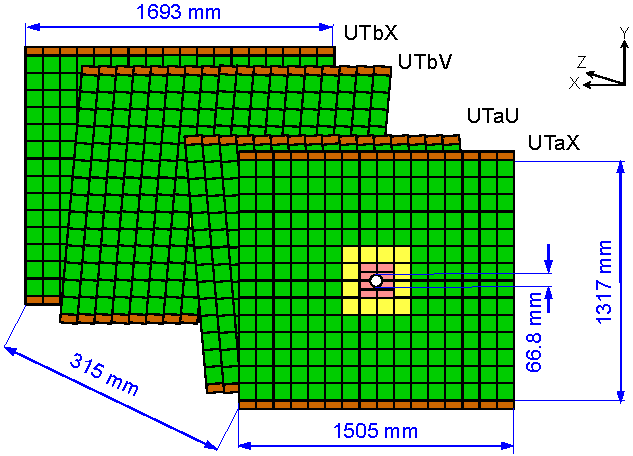
\includegraphics[width=0.7\textwidth]{./figs-lhcb-upgrade-overview/tracking/ut_upgrade.pdf}
    \caption{
        Four detection layers of UT,
        arranged in a $x$-$u$-$v$-$x$ configuration.
    }
    \label{fig:ut-layers}
\end{figure}

\begin{figure}[ht]
    \centering
    \resizebox{0.5\columnwidth}{!}{
        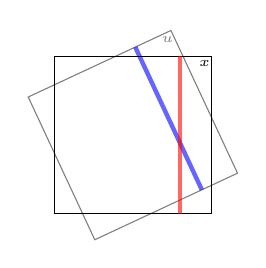
\begin{tikzpicture}
    \begin{scope}[rotate=25]
        % sensor in u plane
        \draw[gray] (1,1) -- (1,-1) -- (-1,-1) -- (-1,1) -- (1,1);
        % the hitting strip
        \draw[blue,ultra thick,opacity=0.6] (0.5,-1) -- (0.5,1);

        \node[text=gray] at (0.91,0.91) {\tiny $u$};
    \end{scope}

    % sensor in x plane
    \draw[black] (1,1) -- (1,-1) -- (-1,-1) -- (-1,1) -- (1,1);
    % the hitting strip
    \draw[red,ultra thick,opacity=0.6] (0.6,-1) -- (0.6,1);

    \node[text=black] at (0.91,0.91) {\tiny $x$};
\end{tikzpicture}

    }
    \caption{
        Illustration of measuring track hit positions with two silicon-strip
        sensors.
        The second sensor is rotated by an angle.
        The intersection between the red and blue strip is the measured position
        of a track.
    }
    \label{fig:strip-sensor-measurement}
\end{figure}

Each detection layer is made of a number of staves,
a vertical structure of sensors and their readout electronics;
the staves are discussed in \cref{ref:ut:overview:stave}.
The sensor readouts are collected by the electronics hosted inside Peripheral
Electronics (PEPI) crates at the top and bottom of the detection layer,
and are described in \cref{ref:ut:overview:pepi}.
Due to space constraints, the low voltage regulators (LVRs),
which supply power to the detector electronics,
are placed farther away from the beam at the service bay;
a brief description of the LVR is given in \cref{ref:ut:overview:lvr}.
An overview of overall UT configuration is shown in \cref{fig:ut-exterior}.

\begin{figure}[!htb]
    \centering

\begin{tikzpicture}
    \node [anchor=south west] (main) {
        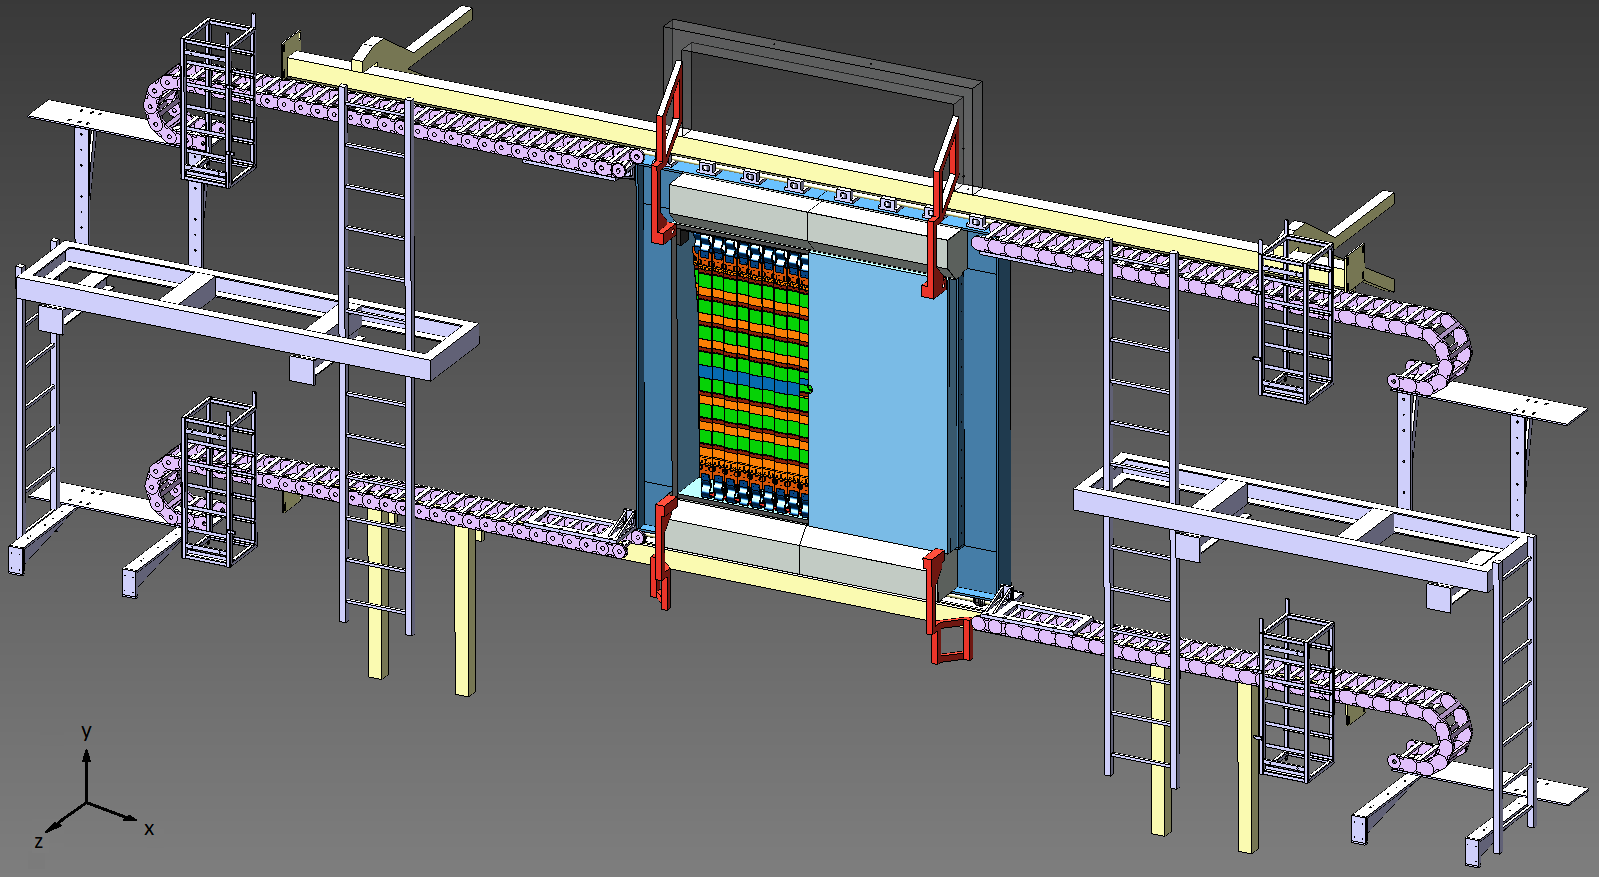
\includegraphics[width=0.88\textwidth]{./figs-ut-upgrade/detector/ut_exterior.png}
    };
    \begin{scope}[x=(main.south east),y=(main.north west)]
        \node[text=white] (A) at (0.7,0.92) {\textbf{PEPI}};
        \node (B) at (0.5,0.71) {};
        \draw[->, thick, draw=white, to path={-| (\tikztotarget)}] (A) edge (B);

        \node[text=white] (C) at (0.3,0.14) {\textbf{Detector box}};
        \node (D) at (0.52,0.52) {};
        \draw[->, thick, draw=white, to path={-| (\tikztotarget)}] (C) edge (D);

        \node[text=white] (E) at (0.7,0.8) {\textbf{Service bay}};
        \node (F) at (0.82,0.74) {};
        \draw[->, thick, draw=white, to path={-| (\tikztotarget)}] (E) edge (F);
    \end{scope}
\end{tikzpicture}

    \caption{
        Overall UT configuration in the LHCb cavern.
        Taken from \cite{Andrews:2018vla}.
    }
    \label{fig:ut-exterior}
\end{figure}


\subsection{Stave}
\label{ref:ut:overview:stave}

Staves consist of four flexible cables (flexes), two on each side,
with sensors and hybrid readout boards wire-bonded on each flex.
These flexes are laid out on a carbon fiber core with CO$_2$ cooling pipes.
The front and back sensors are mounted in a staggered manner to ensure coverage.
The components mentioned above are illustrated in \cref{fig:stave}.

\begin{figure}[!htb]
    \centering
    \begin{subfigure}[t]{0.48\textwidth}
        \centering
        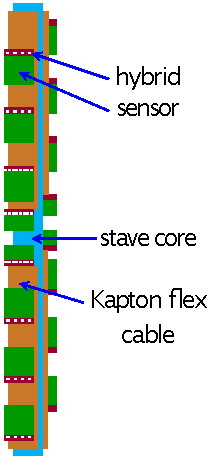
\includegraphics[height=20em]{./figs-ut-upgrade/stave/ut_stave.pdf}
        \caption{
            Schematic of a UT stave.
            Each side of a stave contains two Kapton flex cables.
        }
    \end{subfigure}
    \hspace{10pt}
    \begin{subfigure}[t]{0.48\textwidth}
        \centering
        \includegraphics[width=20em,angle=90]{./figs-ut-upgrade/stave/ut_stave_flex_cable.pdf}
        \caption{
            A signal and power layer of the Kapton flex cable.
            The low voltage coppers are shown in green;
            the data lines are in red.
        }
    \end{subfigure}

    \begin{subfigure}[t]{0.48\textwidth}
        \centering
        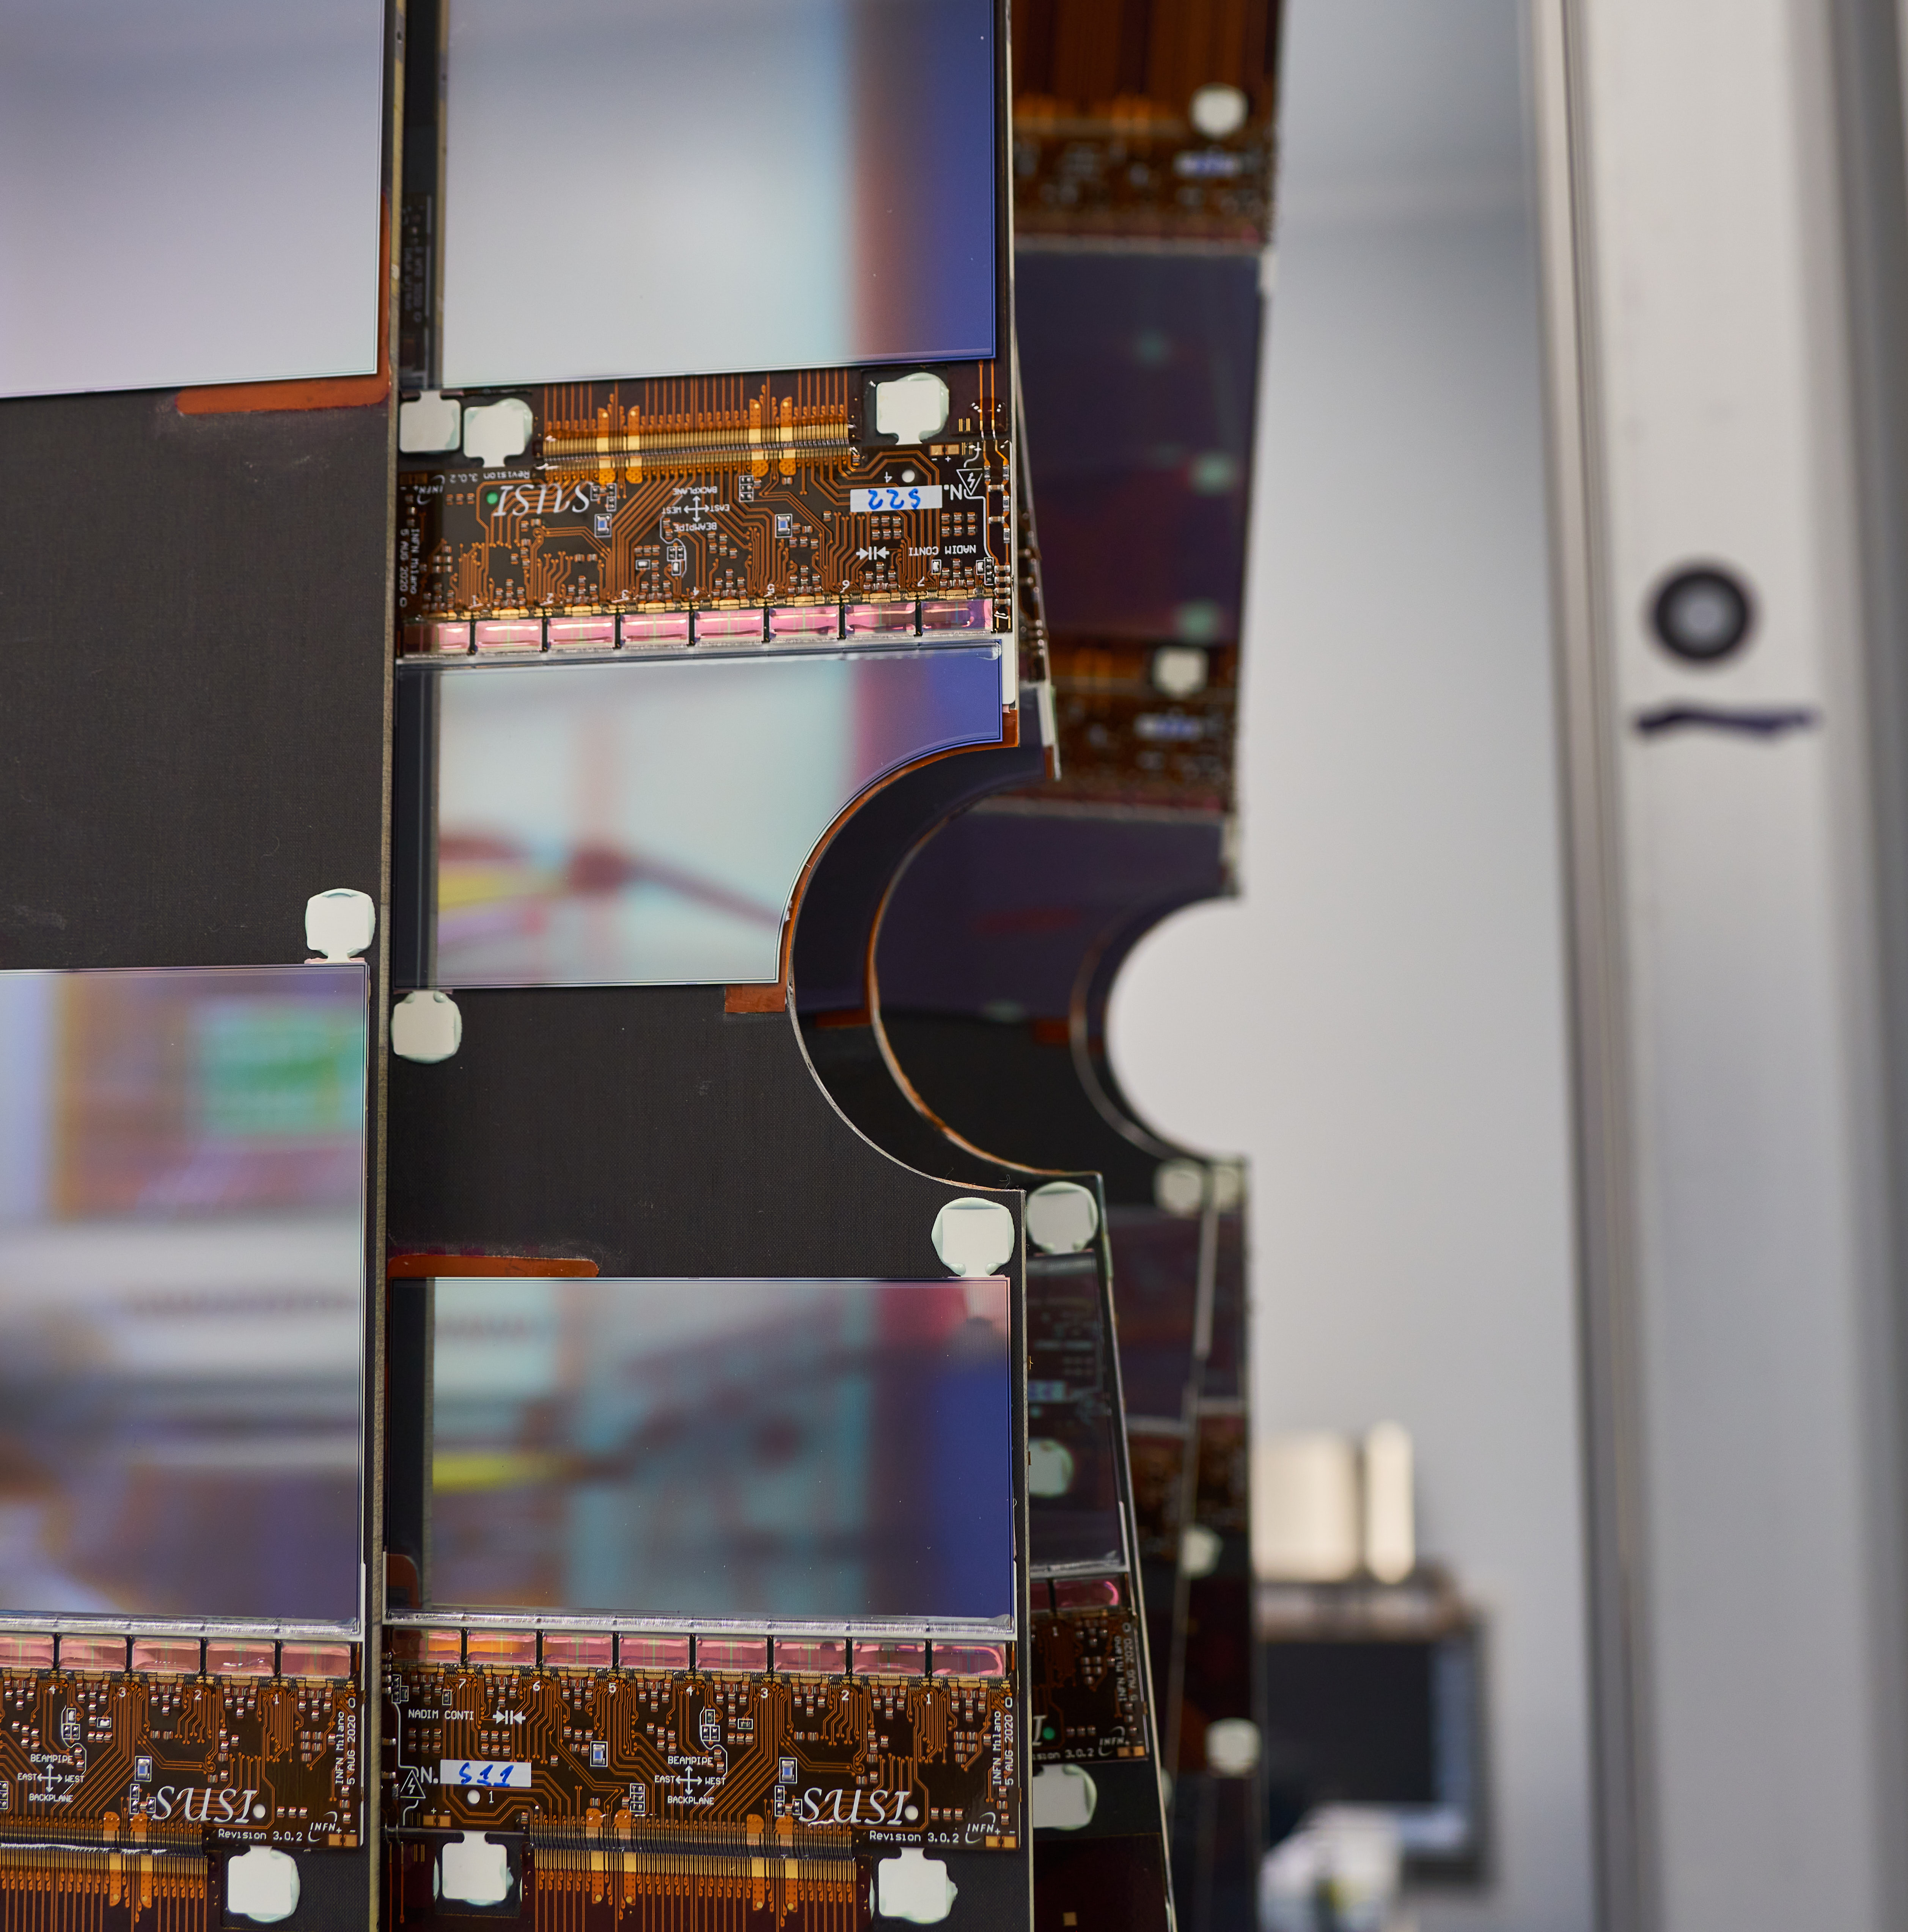
\includegraphics[width=\textwidth]{./figs-ut-upgrade/stave/ut_stave_near_beam_pipe.jpg}
        \caption{
            A stave module with a circular cutout to be placed near the beam
            pipe.
        }
    \end{subfigure}

    \caption{
        UT stave.
    }
    \label{fig:stave}
\end{figure}

There are four types of sensors with different specifications.
The sensors close to the beam pipe (yellow and pink in \cref{fig:ut-layers})
have a finer silicon-strip pitch of 93.5~$\upmu$m and are made with
\emph{n-in-p} process for more radiation hardness,
mainly due to concerns on occupancy and radiation damage.
In addition, the eight half-height sensors (pink) have their strip length halved
to further improve resolution near the beam pipe,
with the four sensors immediately surrounding the pipe having
circular cutouts, instead of rectangular gaps as in TT, to ensure maximum
coverage in the very forward direction.
The outer sensors (green) have a coarser pitch of 187.5~$\upmu$m fabricated with
\emph{p-in-n} technology to reduce cost
\cite{Carli:2783293}.

To minimize the transmission path of the analogue sensor output, readout
SALT ASICs\footnote{
    SALT is developed by the UT collaboration.
    ``ASIC'' stands for Application-Specific Integrated Circuit.
} are glued to a ceramic stiffener along with a sensor and electronic hybrid
circuit to form a single UT module.
The sensor strips are wire-bonded to the input pins of the SALT\footnote{
    SALT ASICs are represented by small white rectangles in
    \cref{fig:ut-layers}.
}
\cite{Wang:2015mem}.
A sample UT module is shown in \cref{fig:ut-module}.

\begin{figure}[!htb]
    \centering
    \begin{subfigure}[t]{0.48\textwidth}
        \centering
        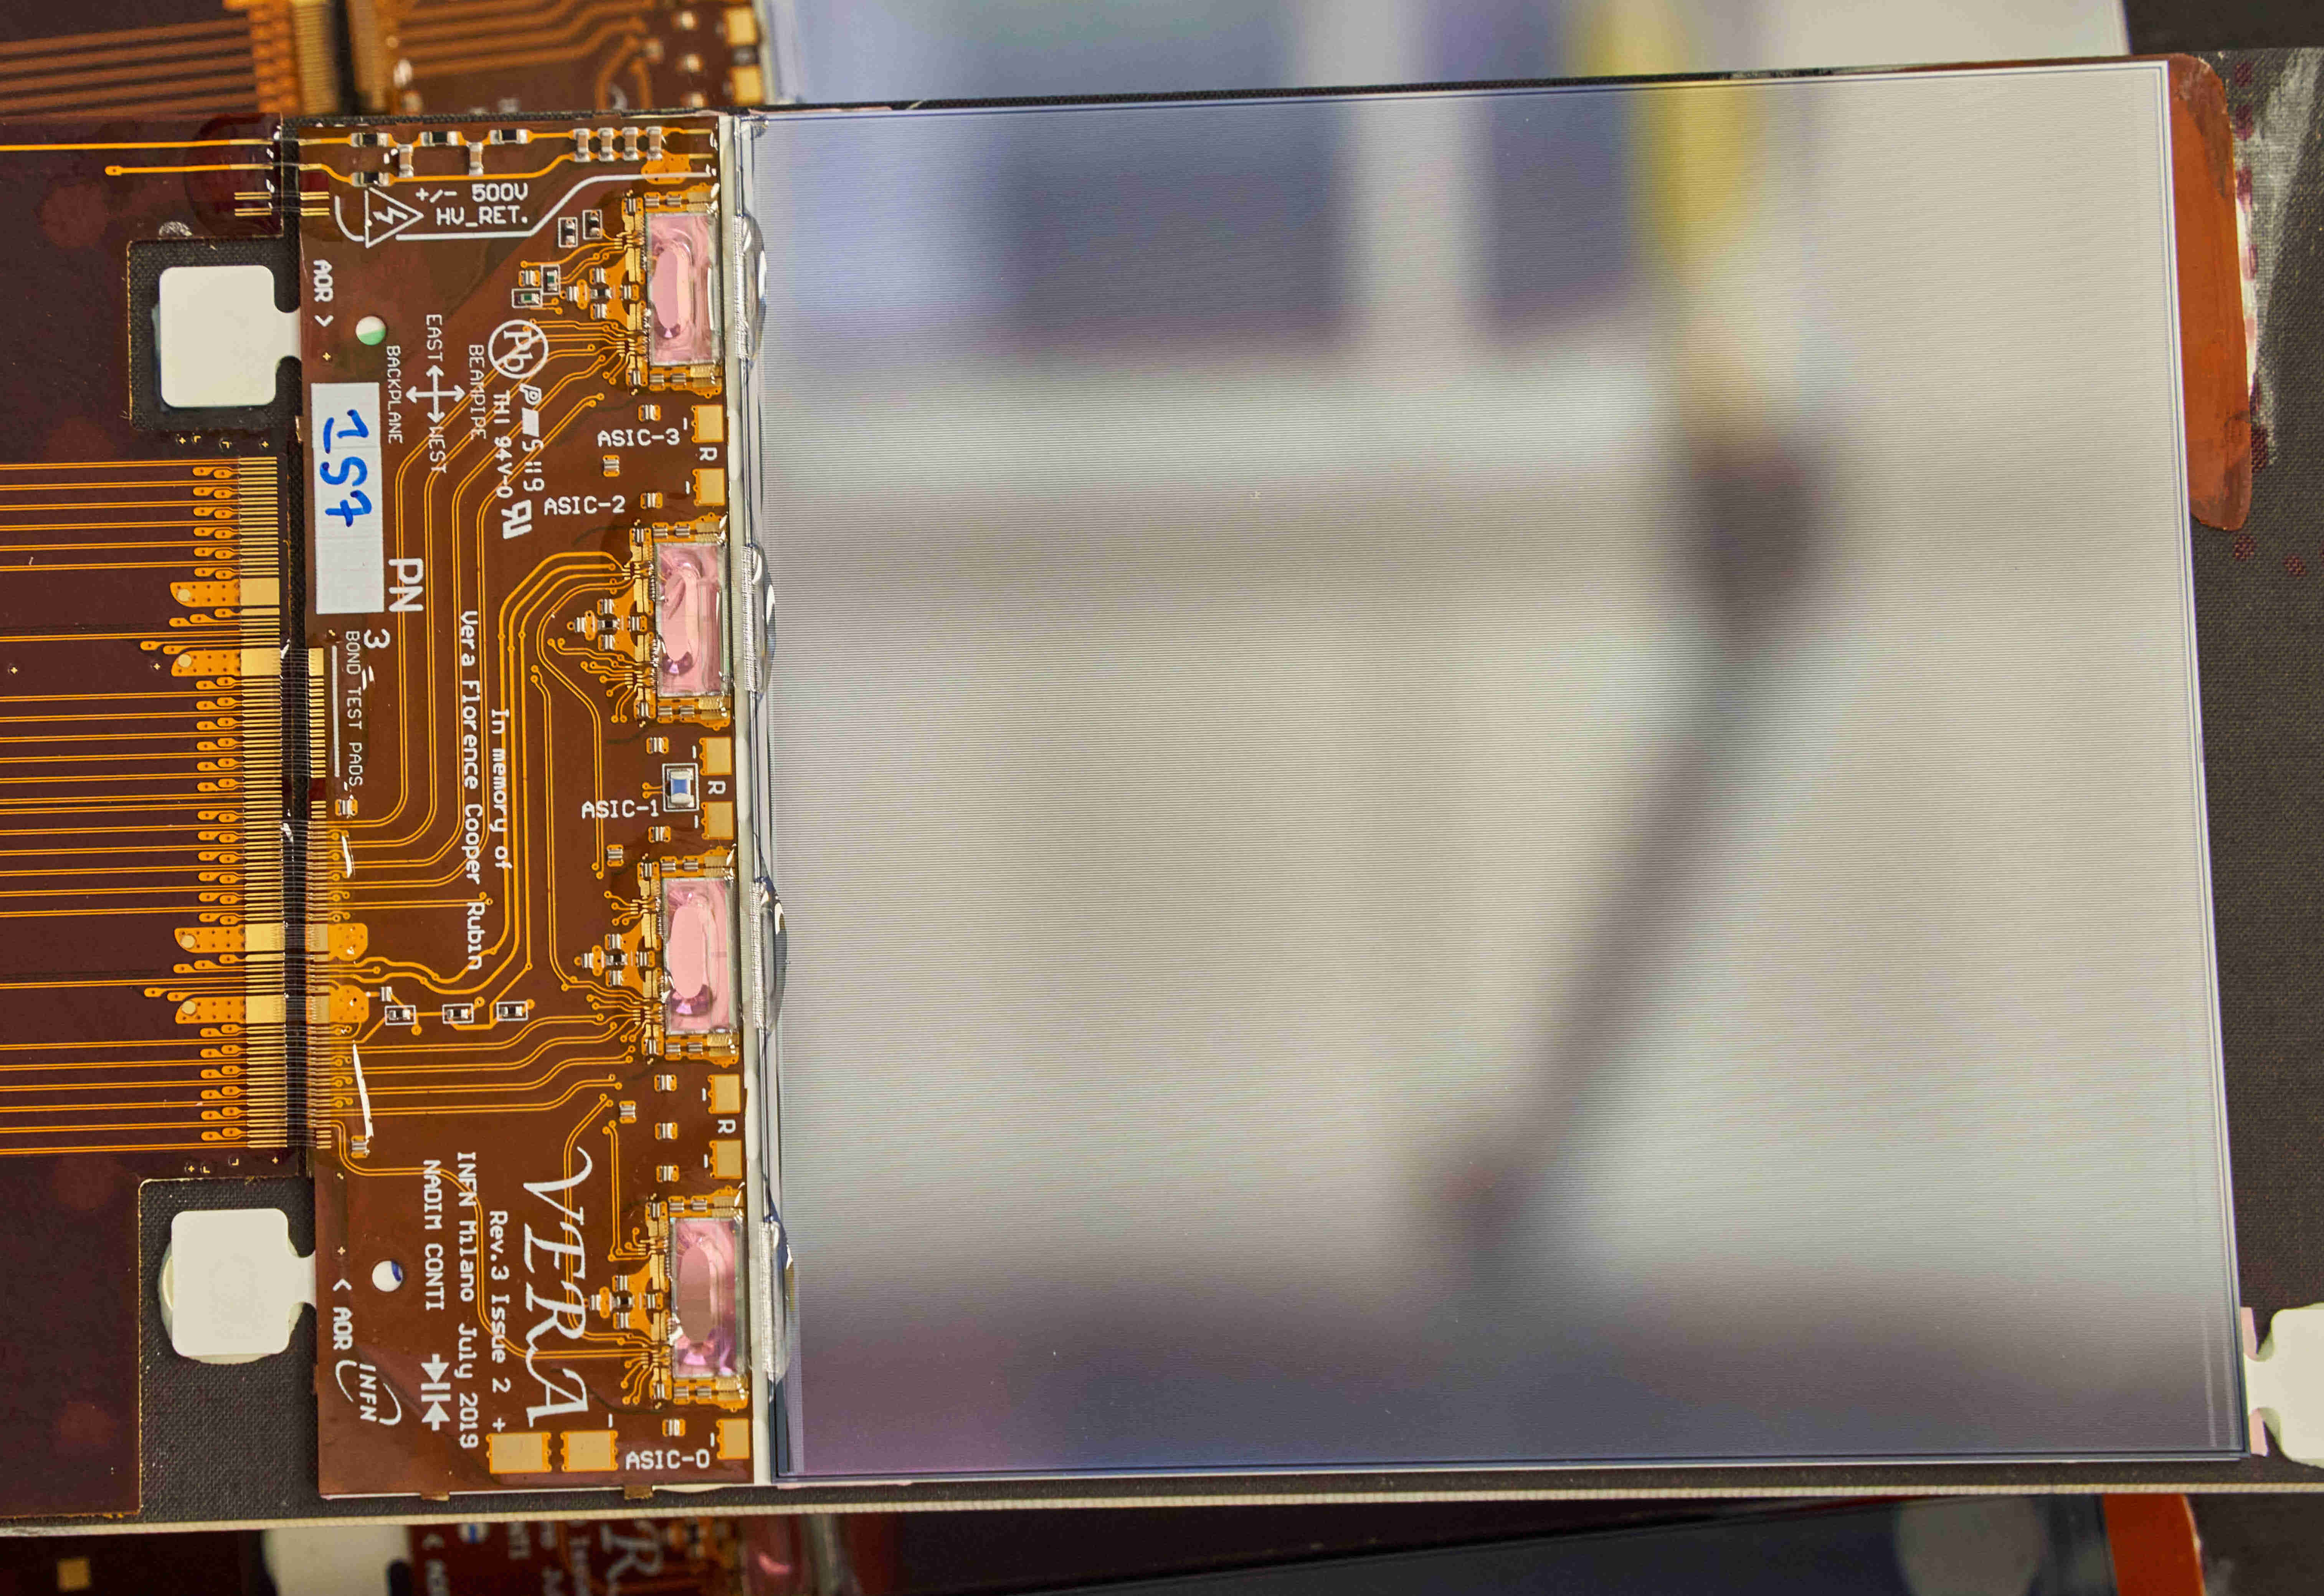
\includegraphics[height=12.5em]{./figs-ut-upgrade/stave/stave_sensors.jpg}
        \caption{
            Full view of a sensor module mounted on a flex.
        }
    \end{subfigure}
    \hfill{}
    \begin{subfigure}[t]{0.48\textwidth}
        \centering
        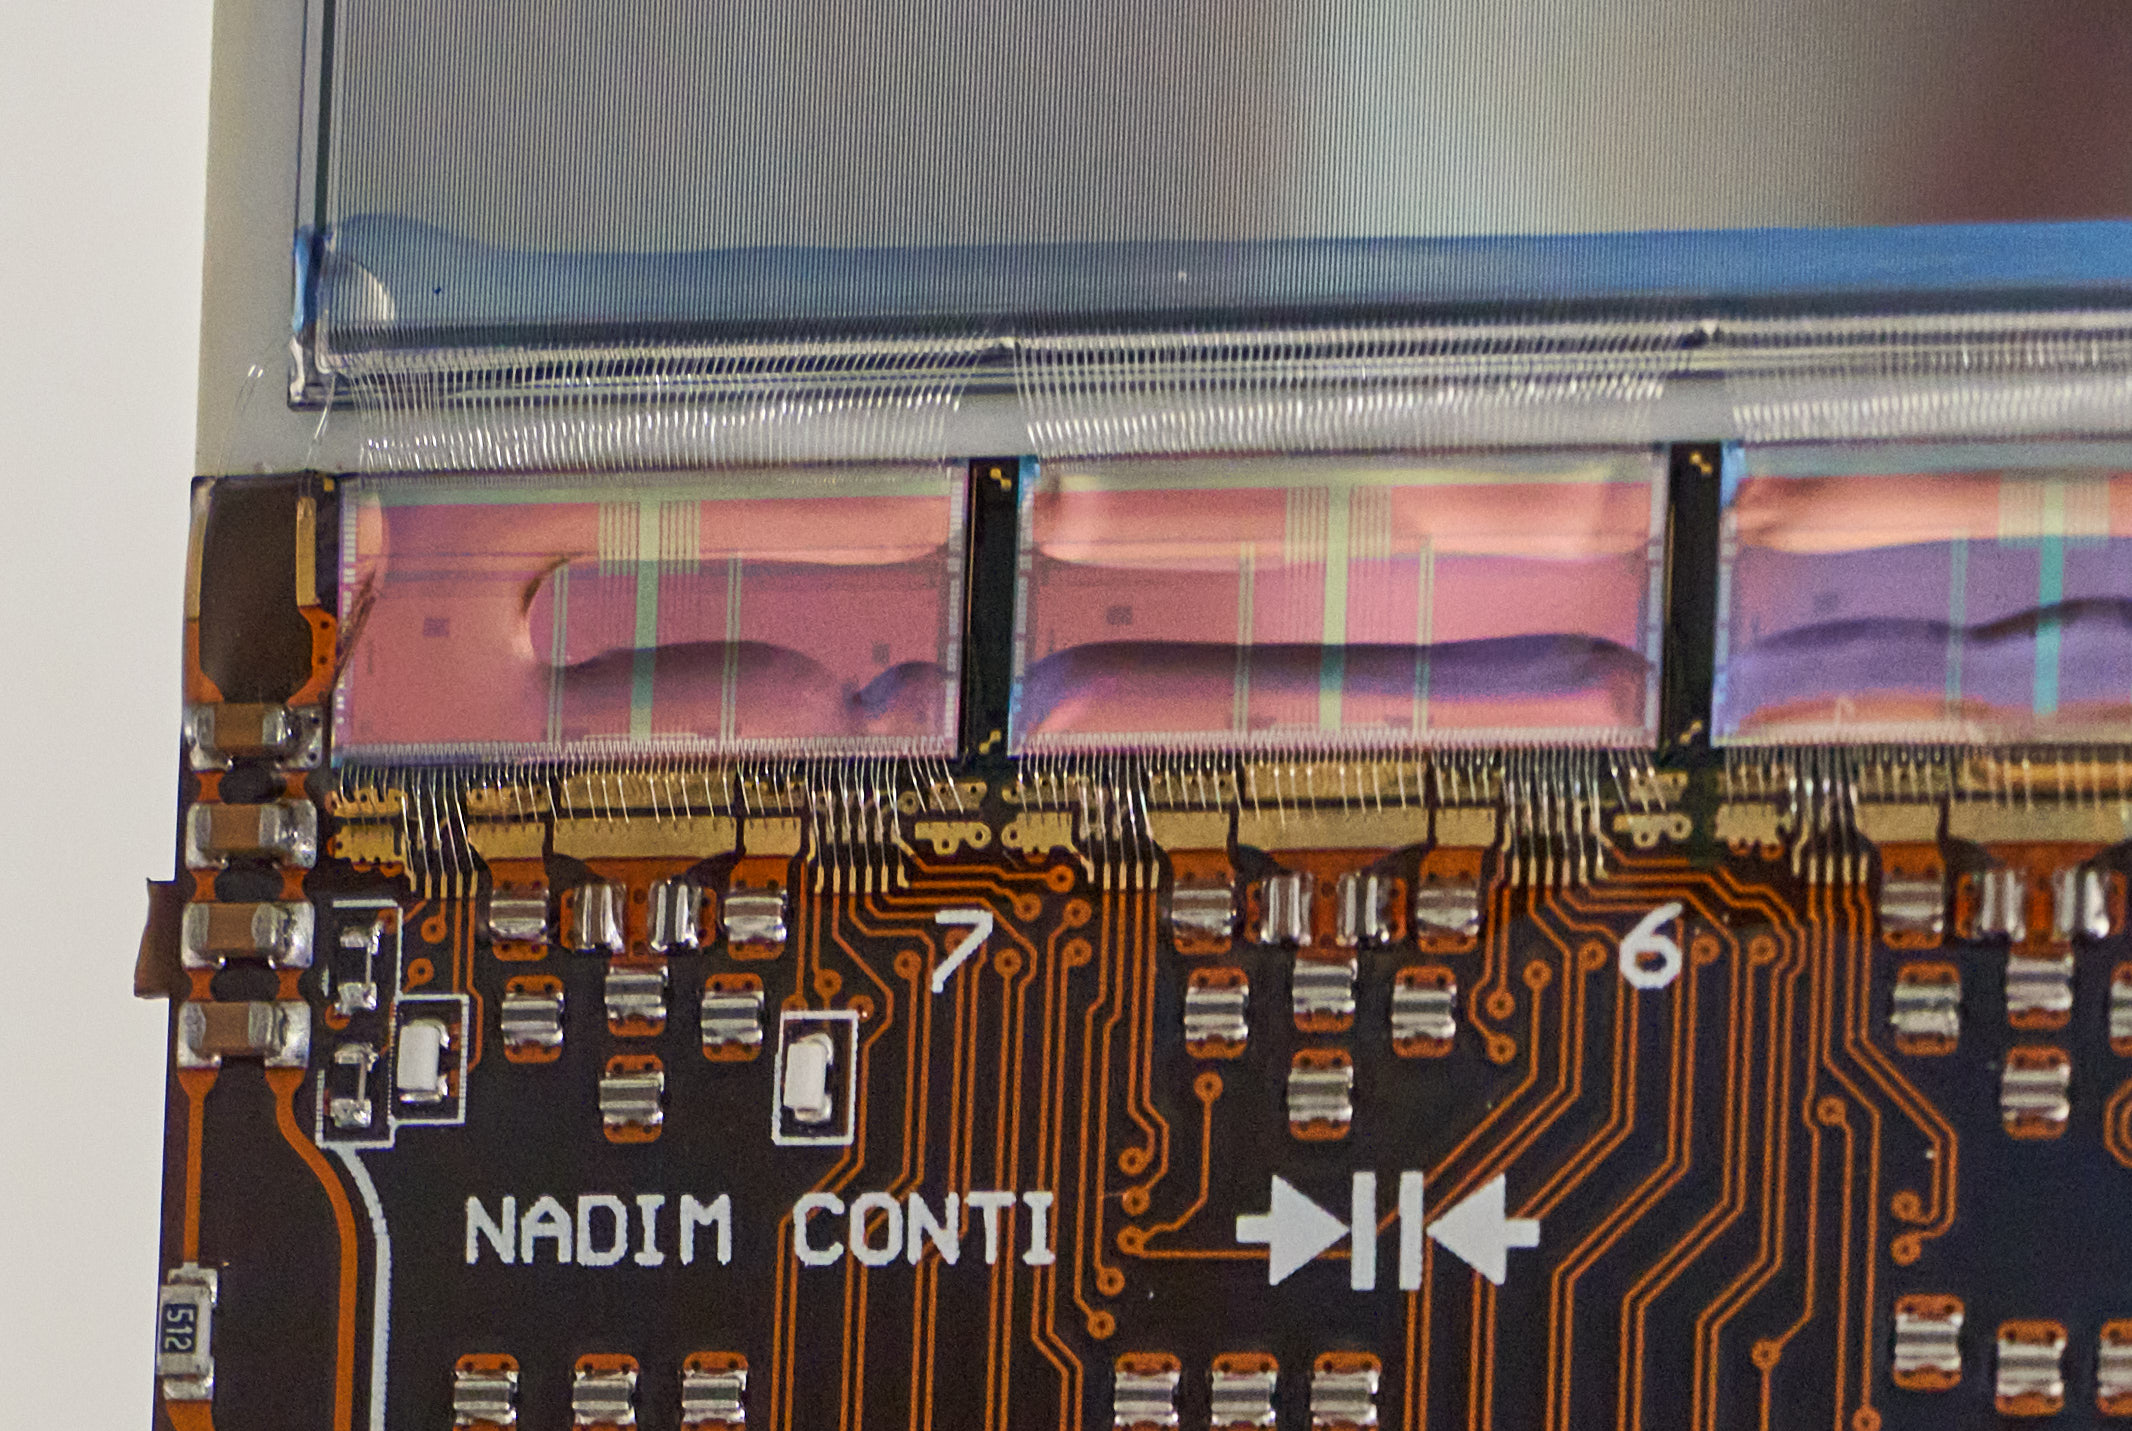
\includegraphics[height=12.5em]{./figs-ut-upgrade/stave/stave_hybrid_closeup.jpg}
        \caption{
            Close-up view on three SALT ASICs glued on a hybrid,
            with their inputs wire-bonded to a sensor.
        }
    \end{subfigure}
    \caption{
        Production sensor modules and SALT ASICs.
    }
    \label{fig:ut-module}
\end{figure}

Fabricated with TSMC 130~nm CMOS process, the SALT ASIC extracts, shapes,
and digitizes analogue signals from the sensor at 40~MHz from 128 channels
simultaneously.
The data is sent out at 320~Mb/s,
which is achieved by increasing the master 40~MHz clock frequency four times
(to 160~MHz) and using double data rate (DDR) transmission.
The master clock is provided by the DCB,
and the frequency increase by a phase-lock loop (PLL).
The SALT chip is capable of generating pseudo-random test patterns on its own
without any excitation on the sensor,
which is employed to test the data transmitting quality.
The chip configuration is set by writing registers via the I2C protocol
\cite{s22010107}.


\subsection{PEPI}
\label{ref:ut:overview:pepi}

Peripheral electronics (PEPI) are responsible for dispatching power to SALTs,
aggregating readout from SALTs to the counting room,
and propagating control commands to the front-end electronics\footnote{
    Front end electronics refer to SALTs and DCBs, which sit close to the beam.
}.
A diagram for data readout and control signal propagation in the UT is displayed
in
\cref{fig:ut-readout-diagram}.

\begin{figure}[!htb]
    \centering
    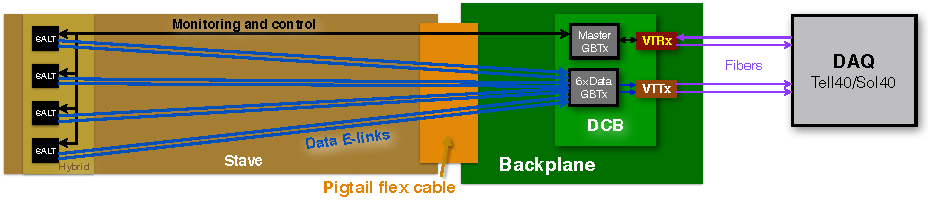
\includegraphics[width=0.85\textwidth]{./figs-ut-upgrade/detector/ut_data_control_flow.pdf}
    \caption{
        UT data and control signal flow diagram.
    }
    \label{fig:ut-readout-diagram}
\end{figure}

Due to space constraint, power, readout data, and control command
are all \emph{dispatched} by a board named Backplane (BP).
Each BP is connected to up to 12 Staves via the Pigtail flex cable,
an engineering marvel on its own\footnote{
    More details regarding the Pigtail can be found in
    \cite{Andrews:2018vla}.
    It is worth noting that during the detector installation,
    very precise bending of the Pigtails are needed to ensure good connectivity.
},
which dispatches power, data, and control signals between the BP and SALTs on
the stave in an \emph{extremely} limited space.
A BP can also host up to 12 DCBs.
Each DCB serializes its input data and convert the digitized electric sensor
readout to an optical one which is then sent to the counting room via fibers.
DCB is also responsible for receiving and translating control commands from the
counting room to both itself and SALT ASICs.
In other words, the whole configurable part of the UT detector is exposed as DCB
registers to the counting room.

PEPI are hosted in PEPI crates, with each containing a single Backplane and up
to 12 DCBs,
as can be seen in \cref{fig:pepi-crate}.
The crate is also responsible for cooling and providing a common ground
reference for all SALTs and DCBs.

\begin{figure}[!htb]
    \centering
    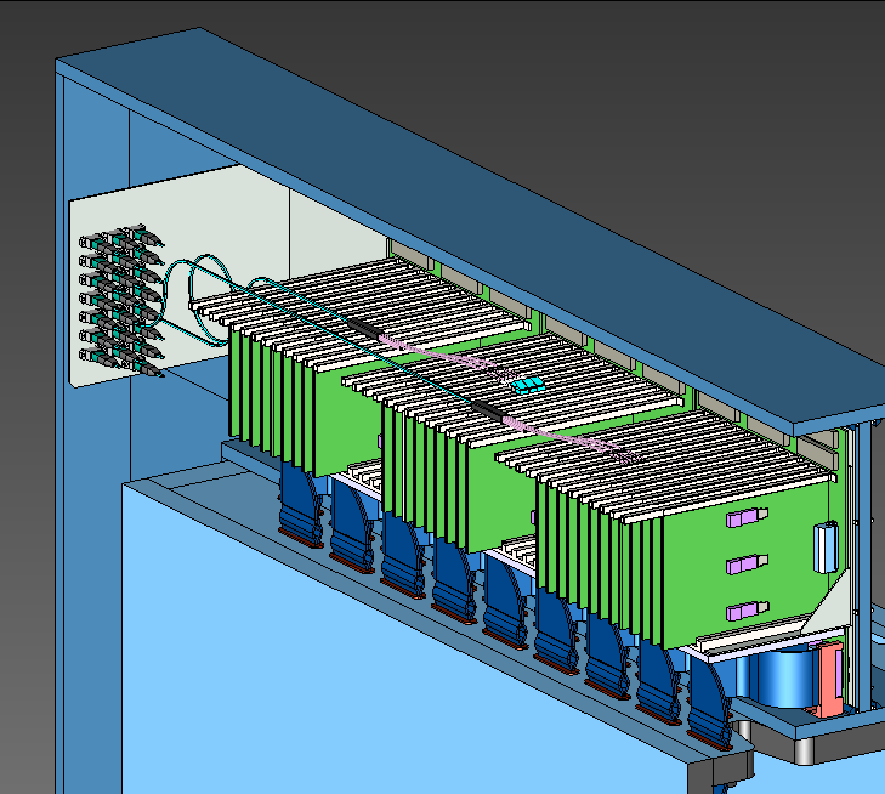
\includegraphics[width=0.7\textwidth]{./figs-ut-upgrade/detector/pepi_crates.pdf}
    \caption{
        A schematic drawing of 3 PEPI crates with DCBs and Pigtails plugged in.
        Taken from \cite{Andrews:2018vla}.
    }
    \label{fig:pepi-crate}
\end{figure}

Backplanes are nothing but a (huge) net of microscopic cables delivering power
and facilitating data exchange to specific connector pins, and contain no active
component (i.e. integrated circuit).
While conceptually simple, Backplanes are extremely hard to route because the
trace density is extremely high.
Fabricated with 28 layers of PCBs\footnote{
    As a reference, a typical motherboard for a desktop PC has 6 layers of PCBs.
}, BPs are at the limit of manufacturability.
To ensure that the traces are routed correctly,
the connectivity map (referred as a ``netlist'') is exported to a
machine-parsable language\footnote{
    One such option exports the netlist to a language that is compatible with
    Common Lisp.
} and checked against a set of pre-defined rules, for example DCBs and
SALTs have differing voltage requirements,
by a Python script.
The quality assurance process of the Backplanes is highly non-trivial, and will
be provided on a separate document by another author.

\begin{figure}[!htb]
    \centering
    \begin{subfigure}[t]{0.48\textwidth}
        \centering
        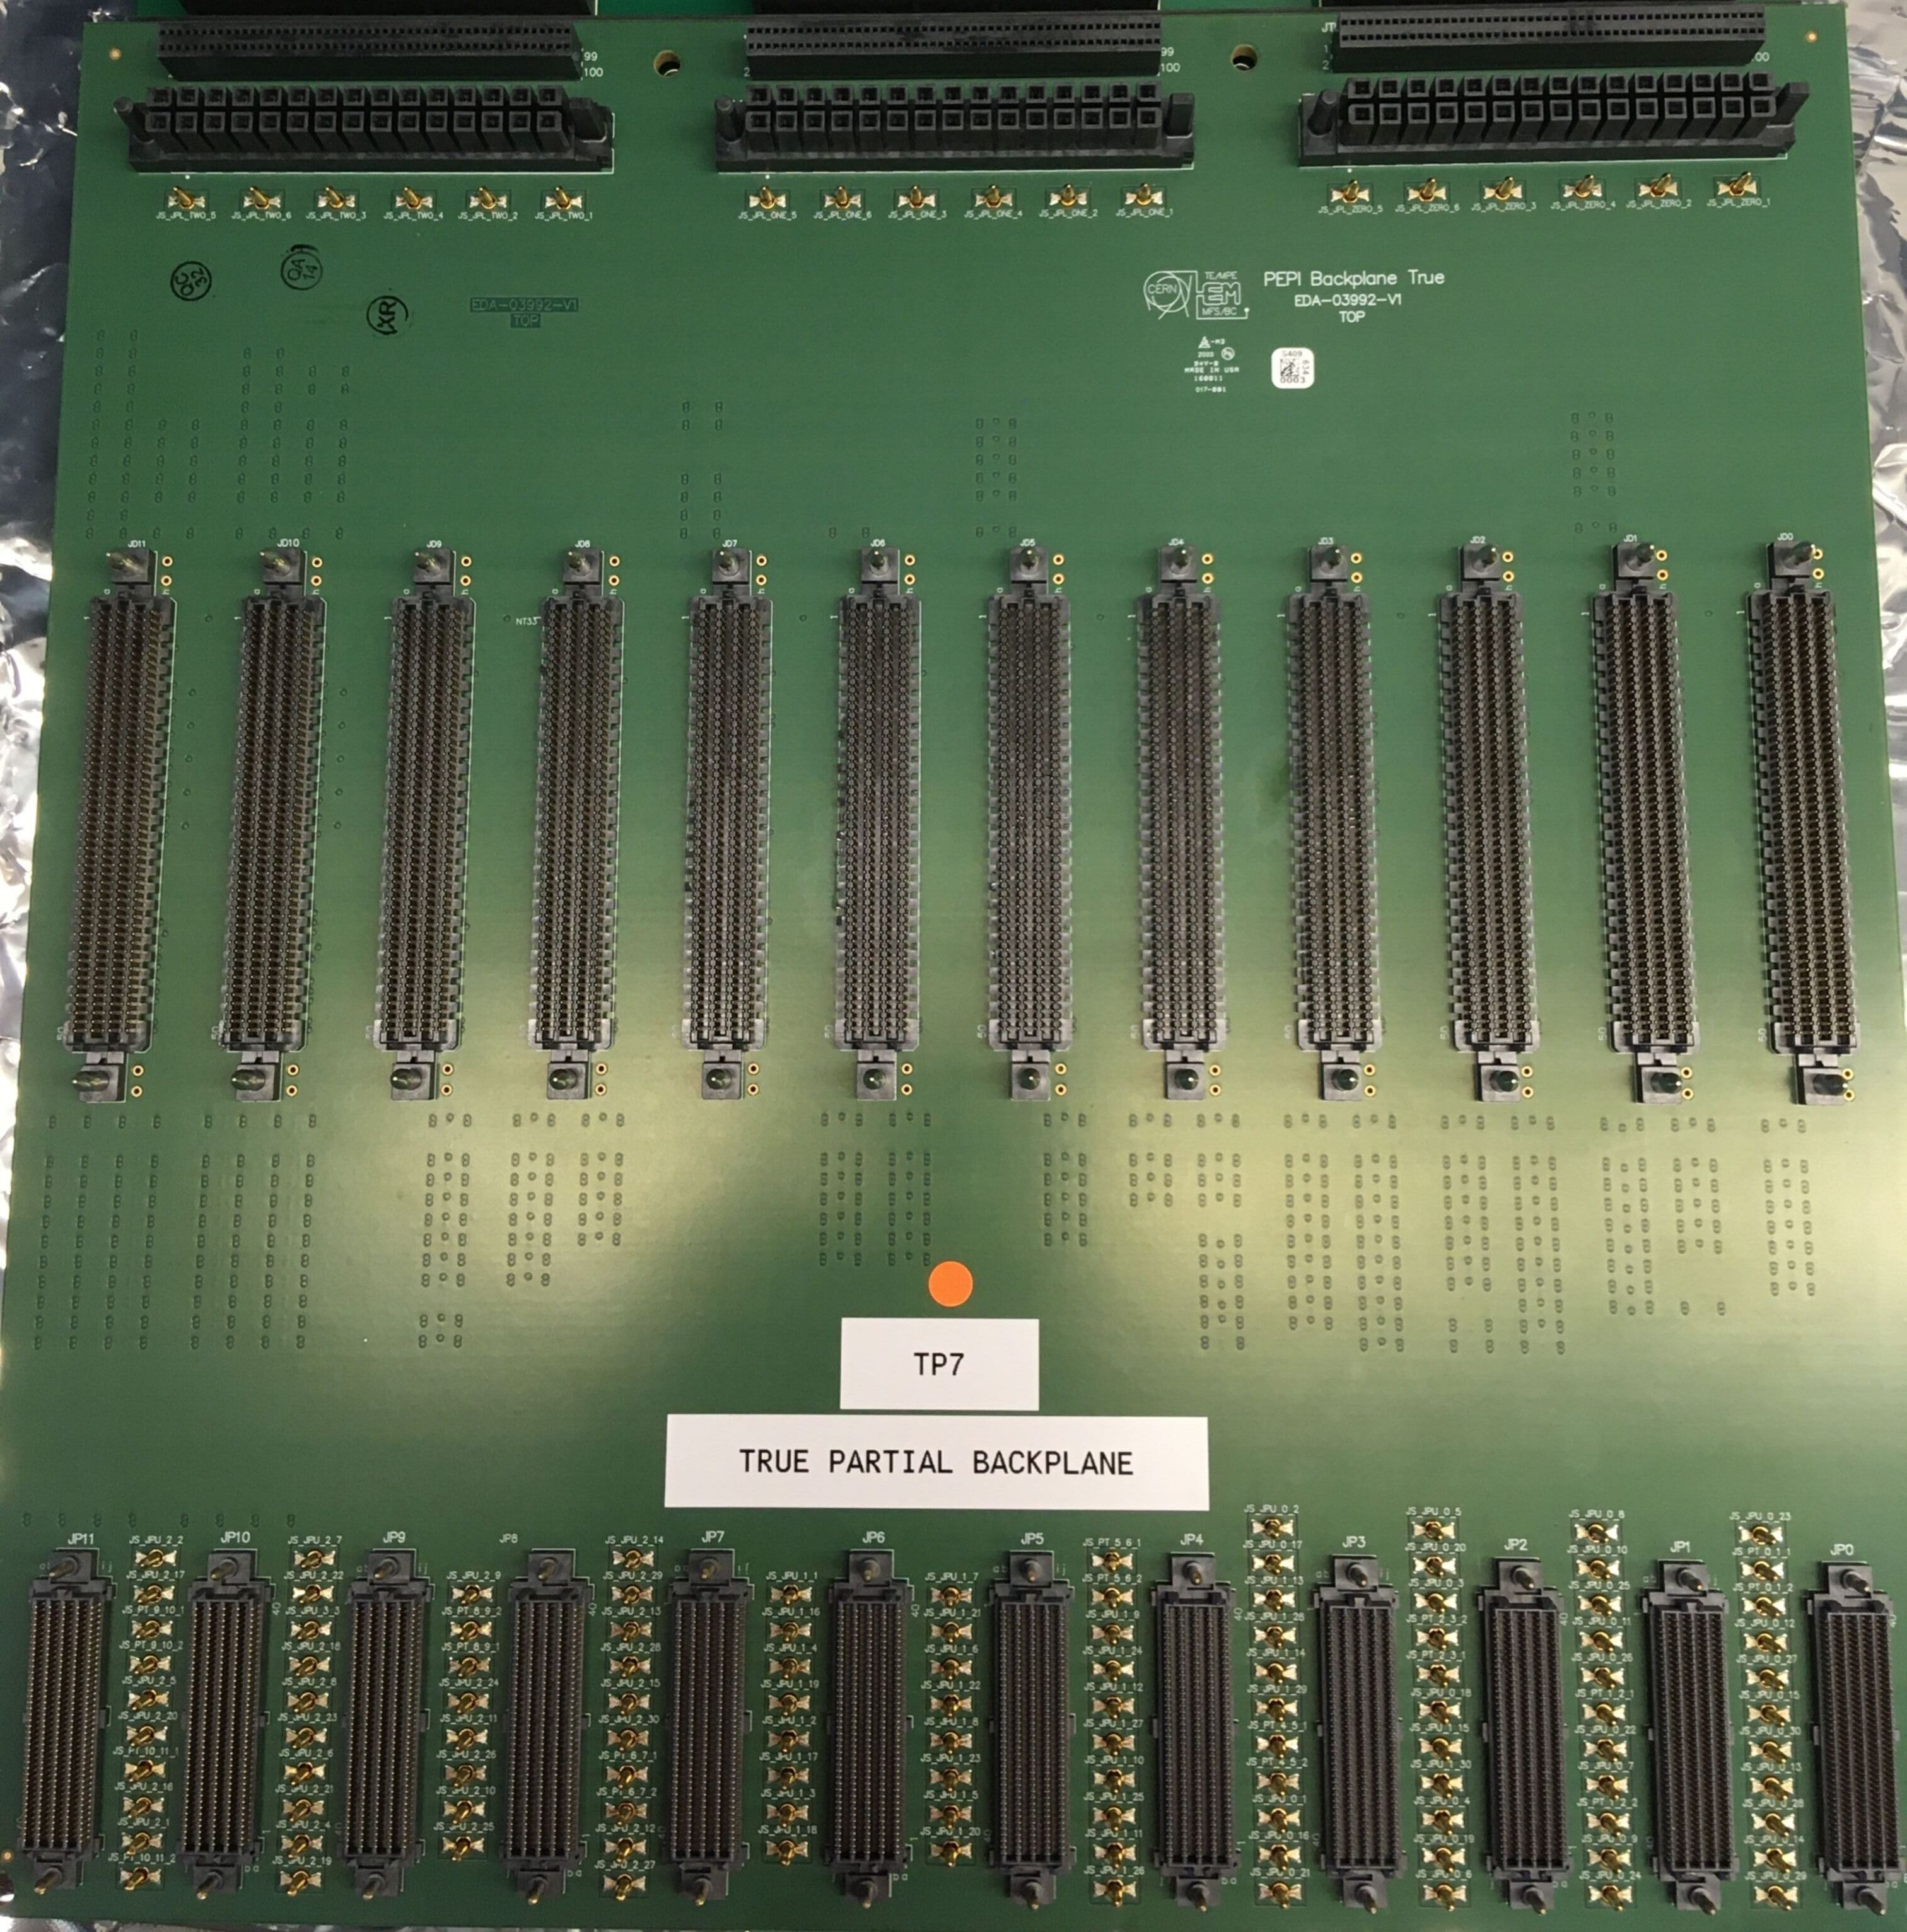
\includegraphics[height=20em]{./figs-ut-upgrade/backplane/backplane_compressed.jpg}
        \caption{
            A production Backplane.
        }
    \end{subfigure}
    \hspace{10pt}
    \begin{subfigure}[t]{0.48\textwidth}
        \centering
        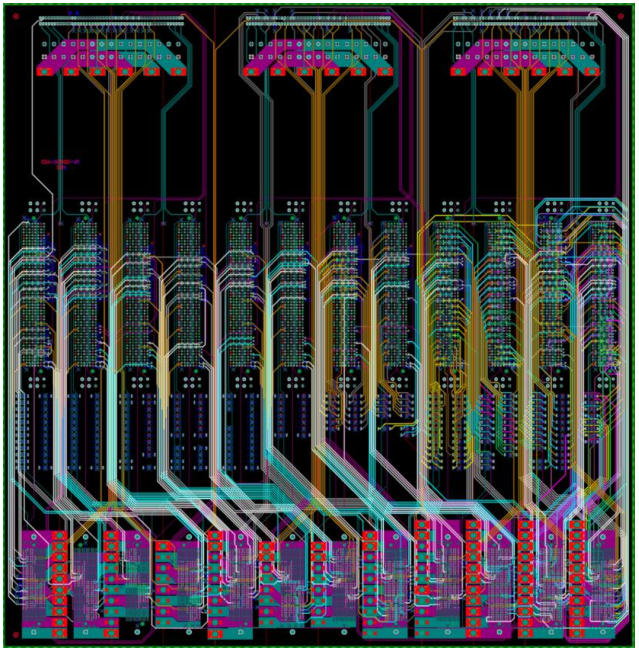
\includegraphics[height=20em]{./figs-ut-upgrade/backplane/backplane_trace.pdf}
        \caption{
            Traces of the backplane are of ultra high density.
        }
    \end{subfigure}

    \caption{
        A production Backplane and its copper trace implement.
    }
    \label{fig:backplane}
\end{figure}

As its name suggests, Data Control Board (DCB) is responsible for aggregating
SALT readouts and propagating slow control commands.
Shown in \cref{fig:dcb-prod}, a DCB is made of 16 layers of PCBs,
and consists of:
\label{dcb-layout}

\begin{itemize}
    \item \textbf{1 master GBTx}:
        Operate in transceiver mode,
        it generates a stable by phase-aligning its on-package quartz oscillator
        clock with the clock signal provided by the readout system,
        and distributes the clock signal to 6 data GBTxs.
        The Timing and Fast Control (TFC) data are distributed to up to 6 SALTs
        it connects to.

    \item \textbf{1 GBT-SCA}:
        Connected to master GBTx via an e-port\footnote{
            The electric port for high-frequency communication with other
            GBT-compatible chips,
            also serves as the building block for e-links.
        },
        the GBT-SCA ASIC connects to the I2C interfaces
        of 6 data GBTx as well as the SALTs.
        It is responsible for relaying slow control commands to these ASICs.
        Also, it is used to read telemetry data,
        namely thermistor readout on SALT, DCB, and optical mezzanines,
        as well as voltages at DCB,
        via its built-in ADC.

    \item \textbf{6 data GBTxs}:
        Operate in simplex transmitter mode with an external clock from the
        master,
        the data GBTxs serialize and scramble the SALT readouts in a way
        suitable for optical transmission.
        The processed signal is sent to a Versatile link module mounted on
        a optical mezzanine for electro-optical conversion and transmission.
        One data GBTx can serialize up to 12 320~Mb/s e-links into a single
        4.8~Gb/s data stream.
        One single data GBTx relays its clock to up to 6 SALTs.

    \item \textbf{1 Versatile link transceiver (VTRx)}:
        An optical transceiver with a GigaBit Laser Driver (GBLD)
        as the electro-optical converter.

        It is used to establish a bi-directional connection to the readout
        system with error-correction functionality that is robust against single
        event upsets (SEU),
        suitable for relaying fast and slow control commands, as well as
        telemetry.

        All Versatile modules are mounted on an optical mezzanine which is
        plugged on DCB.

    \item \textbf{Up to 3 Versatile link transmitter (VTTx)}:
        It contains two GBLDs to establish two uni-directional connections,
        suitable for transmitting serialized SALT readout,
        to the readout system for two data GBTxs.
\end{itemize}

\begin{figure}[!htb]
    \centering
    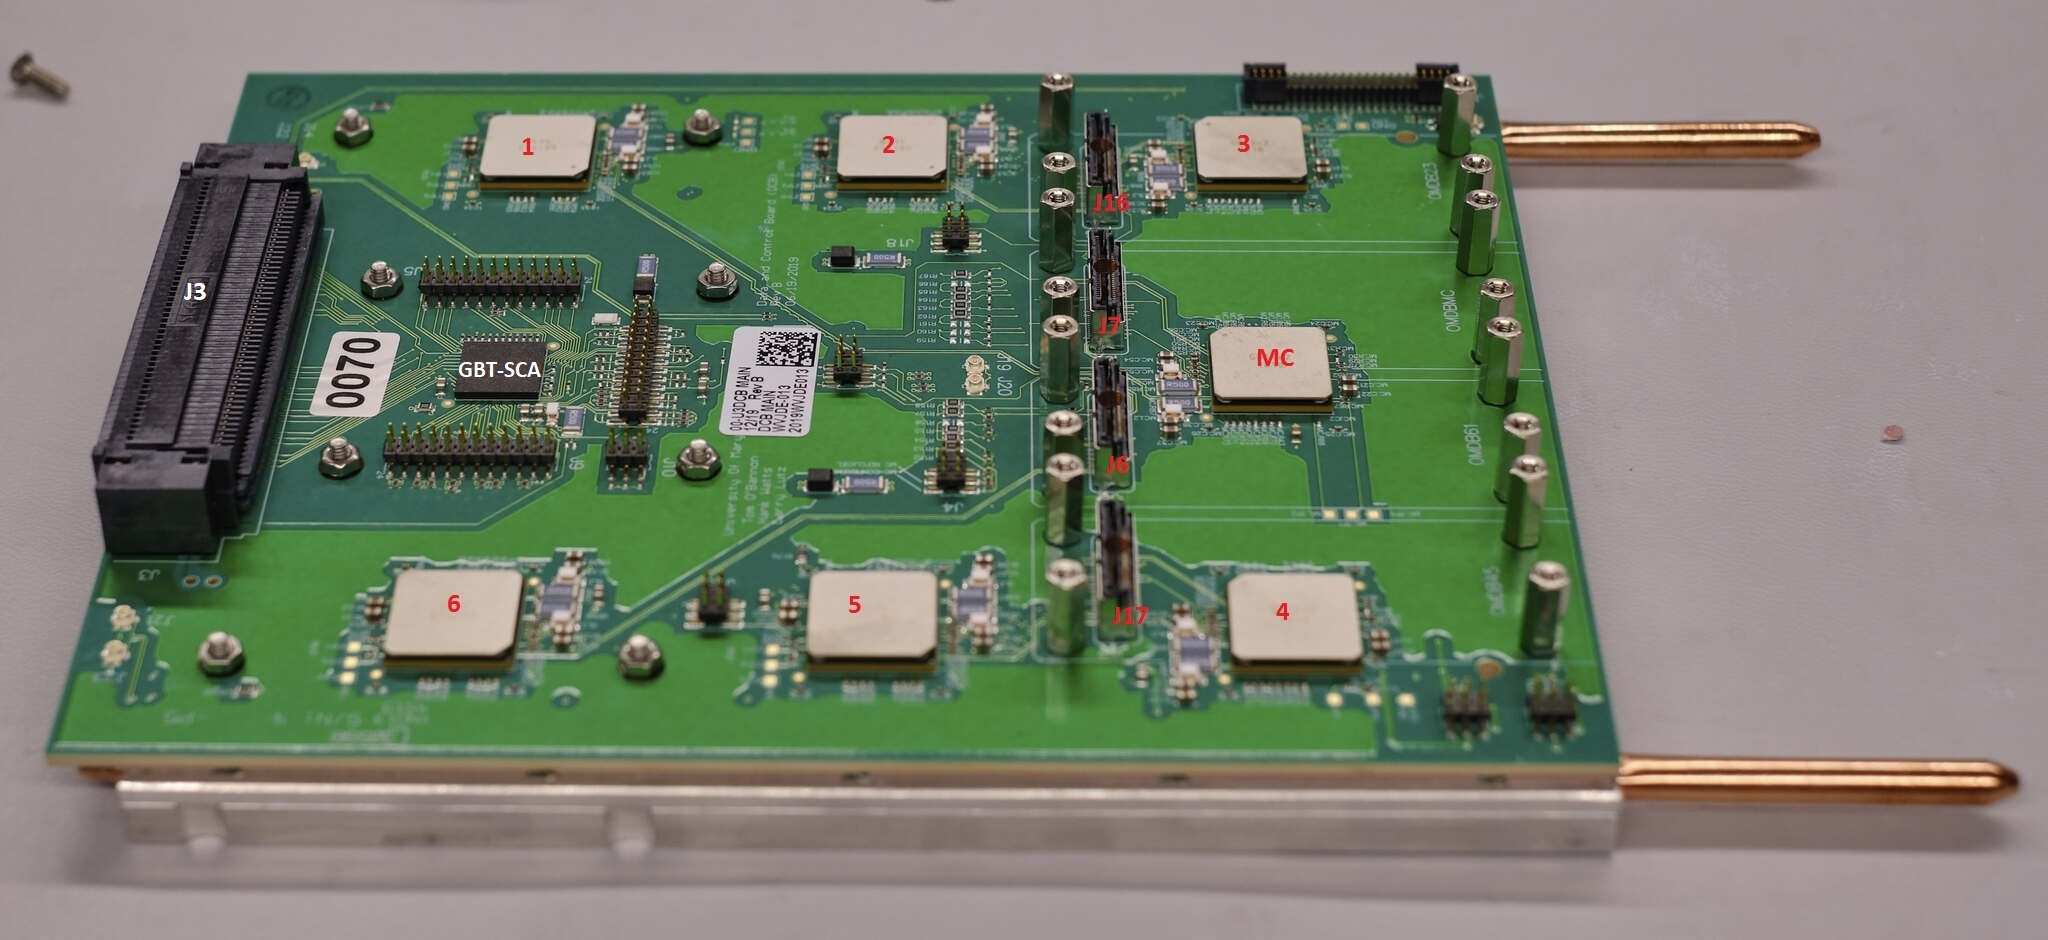
\includegraphics[width=0.8\textwidth]{./figs-ut-upgrade/dcb/dcb_prod.png}
    \caption{
        A production DCB with cooling backplate assembly.
        The master GBTx and GBT-SCA are marked.
        6 data GBTxs are numbered from 1 to 6.
        The BP connector is marked as \texttt{J3}.
        4 optical mezzanine connectors are marked as \texttt{J6, J7, J16, J17}.
        No optical mezzanine is connected.
    }
    \label{fig:dcb-prod}
\end{figure}

As the author spent quite some time to test (and to make sense) of the
DCBs, more information regarding DCBs will be provided in \cref{ref:ut:dcb}.


\subsection{LVR}
\label{ref:ut:overview:lvr}

Installed inside service bays, the Low Voltage Regulator (LVR),
shown in \cref{fig:lvr},
delivers power
to the SALTs and DCBs with a $\sim 10$~m long cable
which makes the resistance of the cable non-ignorable.

\begin{figure}[!htb]
    \centering
    \begin{subfigure}[t]{0.48\textwidth}
        \centering
        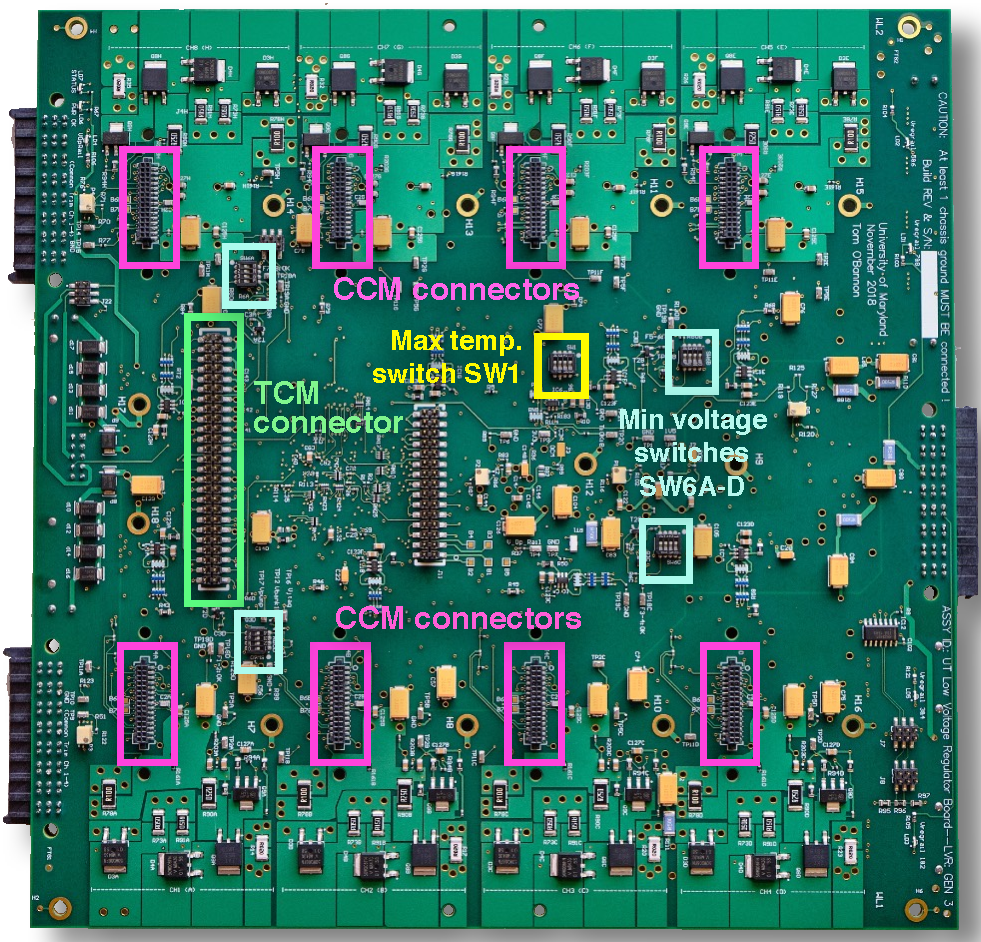
\includegraphics[width=0.87\textwidth]{./figs-ut-upgrade/lvr/lvr_top_view.pdf}
        \caption{
            LVR top view (CCM/TCM side).
        }
    \end{subfigure}
    \hfill
    \begin{subfigure}[t]{0.48\textwidth}
        \centering
        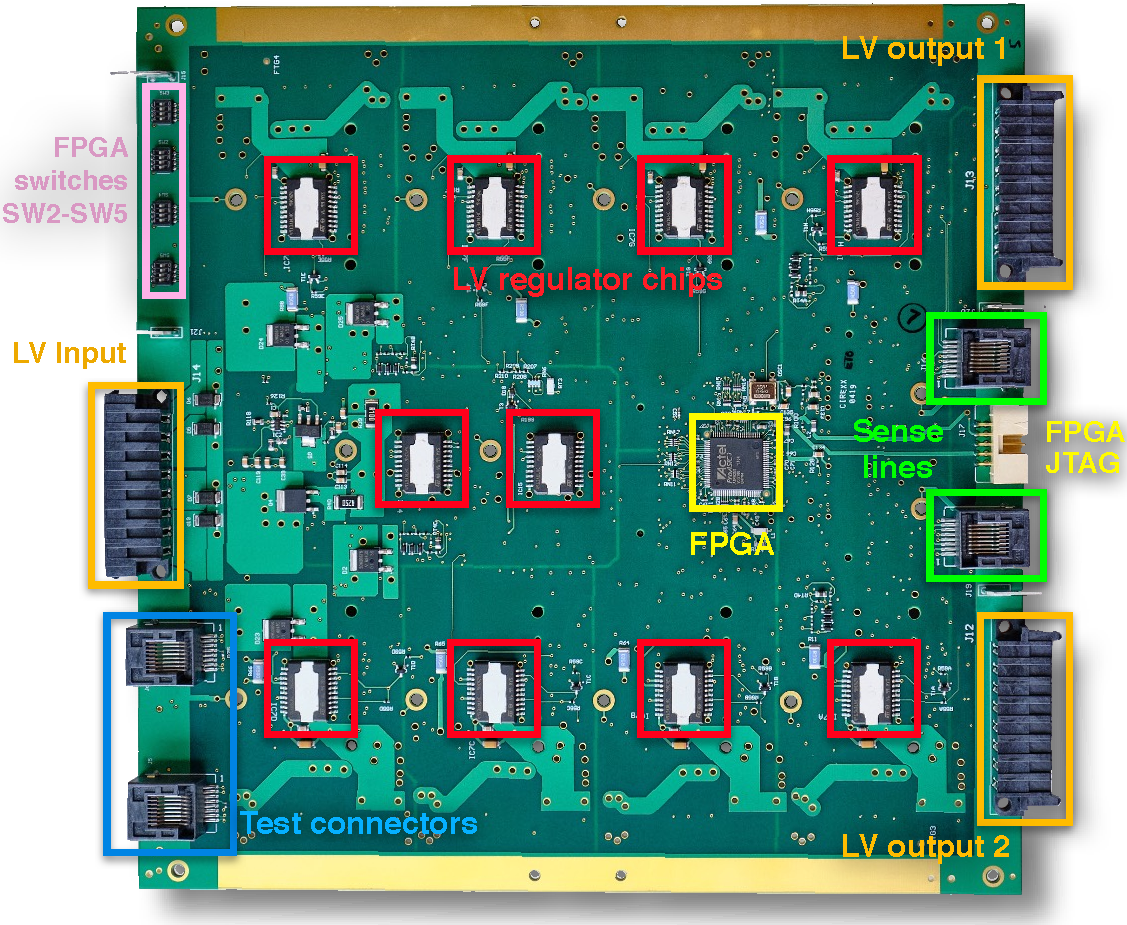
\includegraphics[width=\textwidth]{./figs-ut-upgrade/lvr/lvr_bot_view.pdf}
        \caption{
            LVR bottom view (FPGA side).
        }
    \end{subfigure}

    \caption{
        A LVR.
        Taken from \cite{LVR_manual}.
    }
    \label{fig:lvr}
\end{figure}

To ensure correct voltages are delivered at the ASIC side,
LVR implements a remote sensing capability by a Microsemi FPGA such that the
remote voltage is constantly monitored and kept at the specified
voltages\footnote{
    Consider the specified voltage is at 1.25~V, the LVR output voltage is
    at about 1.4~V.
    The $V_\text{sense}$ vs. $V_\text{LVR}$ lookup table can be found at
    \cite{LVR_output_voltage_lookup}.
}, which require one pair of sense lines carrying little current in addition to
the pair of current
carrying lines (4 lines for a single output channel).
It can be intuited as if LVR can probe with a multimeter at the power input of
the front-end electronic and adjust its output voltages accordingly.
When the sense line breaks, the unsensed output voltage at LVR side is always
at the specified value so ASICs will be undervolt, which is safe.
However, when the sense line is shorted, LVR will keep ramping up the voltage
up to 5.5~V which will fry the ASICs for sure.
Thus particular care is taken during the cabling phase to ensure no such short
happens.

One LVR has up to 8 output channels; each is configured by a Channel
Configuration Mezzanine (CCM) with which the specified voltage is defined by a
potentiometer.
There are three voltage specifications: SALT requires 1.25~V; DCB GBTx requires
1.5~V; the Versatile modules require 2.5~V.
A single channel can output up to 2.5~A of current.
When more current is needed, two channels can be configured into a master-slave
pair in which case the sense lines from the master channel dictate the output
of the pair.

Remote channel control and monitoring via the SPI protocol is also implemented
by the FPGA;
such functionality can be accessed via the Telemetry Control Mezzanine (TCM)
connector.
A separately designed TCM board integrates the LVR into the LHCb control system.

More information regarding LVRs can be found at \cite{LVR_manual}.


\section{The Data Control Board (DCB)}
\label{ref:ut:dcb}

DCB is part of an implementation of the reference LHCb front-end  electronic
module.
Shown in \cref{fig:lhcb-ref-fe},
a complete LHCb front-end electronic device contains digitization of sensor
readout, serialization of digitized readout, and distribution of control
commands.
The DCB,
schematically shown in \cref{fig:dcb-schematic},
implements the last two functionalities (for UT the sensor readout is implemented
by the SALT ASIC).

\begin{figure}[!htb]
    \centering
    \begin{subfigure}[t]{0.46\textwidth}
        \centering
        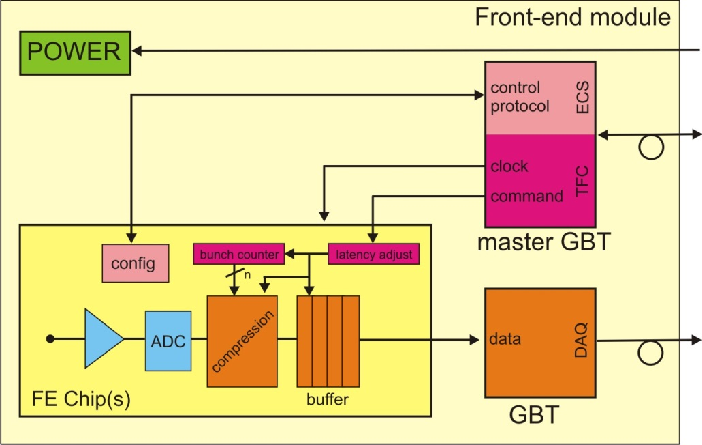
\includegraphics[height=12em]{./figs-ut-upgrade/dcb/lhcb_ref_fe.pdf}
        \caption{
            The LHCb reference design for front-end electronics.
            Taken from \cite{Wyllie:2011sya}.
        }
        \label{fig:lhcb-ref-fe}
    \end{subfigure}
    \hfill
    \begin{subfigure}[t]{0.46\textwidth}
        \centering
        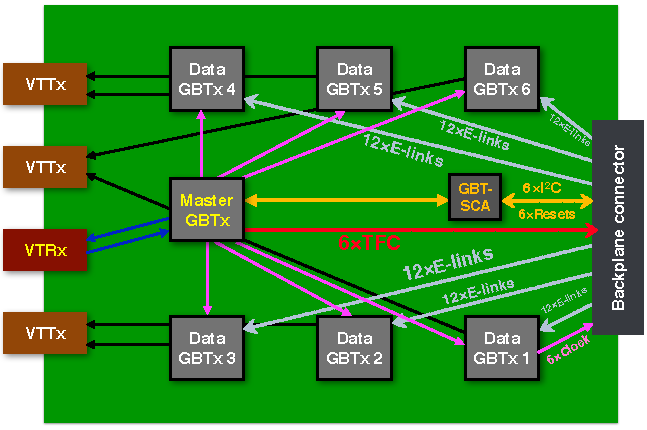
\includegraphics[height=12em]{./figs-ut-upgrade/dcb/dcb_schematic.pdf}
        \caption{
            Schematic DCB layout.
        }
        \label{fig:dcb-schematic}
    \end{subfigure}

    \caption{
        Comparison between the reference LHCb front-end electronic and DCB.
    }
\end{figure}

The physical layout of the DCB has been summarized in \cref{dcb-layout}.
The rest of the section provides more information
on the GBT architecture which is the foundation of DCB
(\cref{dcb-gbt,dcb-gbt-link,dcb-elink}),
the operation of DCB (\cref{dcb-init}),
and the testing and quality assurance of DCB (\cref{dcb-test-data,dcb-qa}).
More details about configuring DCB can be found in a document
(not publicly available yet) prepared by the Maryland group.


\subsection{The GBT chipset}
\label{dcb-gbt}

The GigaBit Transceiver (GBT) architecture is developed by CERN to provide a
high-speed optical data transmission solution capable of operating in a
highly radiative environment, such as in LHC \cite{P_Moreira_2010}.
The following ASICs from the GBT project are used in DCB:

\begin{itemize}
    \item \textbf{GBTx}:
        GBTx is a radiation tolerant serializing/deserializing ASIC for
        implementing high-speed uni- or bi-directional optical links in high
        energy experiments
        \cite{gbtx_manual}.

    \item \textbf{GBLD}:
        GigaBit Laser Driver:
        A configurable VCSEL\footnote{
            Vertical-cavity surface-emitting laser.
            It has many modern applications such as in computer mice and optic
            fiber communication.
            The technical details is unknown to the author but is irrelevant
            for the topic.
        } driver
        \cite{gbld_manual}.

    \item \textbf{GBT-SCA}:
        GigaBit Transceiver-Slow Control Adapter provides an interface between
        various industrial-standard slow control protocols,
        namely SPI, I2C, JTAG, and GPIO, to the GBT link protocol.
        It also has a built-in multi-channel ADC that can be configured and
        read via the GBT link \cite{sca_manual}.
\end{itemize}


\subsection{The GBT link}
\label{dcb-gbt-link}

The GBT link has two transmission mode relevant for DCB: FEC and widebus mode.
The former provides error correction capability with the trade-off of reduced
data transfer speed at 3.36~Gb/s,
making this mode suitable for carrying out critical timing and control data.
The latter works at 4.48~Gb/s without error correction at link level,
and is used for readout data transmission.
In either mode, a single data frame is always 120 bit long.

\paragraph{Transceiver}
The master GBTx is configured to work in the transceiver mode, working in
FEC mode.
Each frame in this mode contains the following fields:

\begin{itemize}
    \item \textbf{Header}:
        8 bits.
        For delimitation (identification) of frame boundaries
        (frame synchronization).

    \item \textbf{Internal Control (IC)}:
        2 bits.
        Reserved for remote provisioning
        (i.e. change selected configuration registers and read telemetry
        information) of the master GBTx.

    \item \textbf{External Control (EC)}:
        2 bits.
        Reserved for transferring external slow control commands,
        such as I2C commands, to the GBT-SCA.
        Both IC and EC has a fixed speed of 80~Mb/s.

    \item \textbf{Data}:
        80 bits.
        Contain 5 e-link groups, each 16 bits long (2 Byte).
        At 320~Mb/s data rate, each e-link group has 2 e-links.

    \item \textbf{Forward Error Correction (FEC)}:
        32 bits.
        The error correction algorithm uses a 2-time interleaved Reed-Salomon
        $RS(15, 11)$ code with 4-bit symbols.
        In practice the data is robust against up to 16 consecutive bit
        corruptions.

        All fields above are protected by the FEC field.
\end{itemize}

\paragraph{Transmitter}
Each data GBTx transmitter operates in the widebus mode.
A widebus frame is identical to a FEC frame except that it has no FEC field and
extends the data field to 112 bit so that the total number of e-link groups is
increased to 7.
As a trade-off, there is no error correction capability at link level.

As can be seen from the structure of the GBT frame, there is an overhead
due to header and IC/EC fields.
This is why the data transmission speed is at 4.48~Gb/s instead of 4.8~Gb/s.


\subsection{E-links}
\label{dcb-elink}

As described in the previous section,
operating in widebus mode,
a data GBTx can provide up to $2 \times 7 = 14$ e-links\footnote{
    A GBTx contains many e-ports which are used to facilitate e-links.
},
duplex local electric serial links implemented with low-voltage differential
pairs transmitting data at 320~Mb/s
\cite{gbtx_manual},
with the transmission speed chosen by the design of the SALT.
In DCB, however, only up to 12 e-links per data GBTx are accessible to the
SALTs.

A SALT requires 3--5 e-links \cite{s22010107},
so a single data GBTx can aggregate readout data from up to 4 SALTs.
The allowed SALT-e-link combinations are listed in \cref{tab:salt-elink}.

\begin{table}[!htb]
    \centering
    \begin{tabular}{ c | c }
        \toprule
        \textbf{Number of SALTs} & \textbf{e-links per SALT} \\
        \midrule
        4  &  3  \\
        2  &  3  \\
        2  &  4  \\
        2  &  5  \\
        \bottomrule
    \end{tabular}

    \caption{Possible SALT-e-link combinations.}
    \label{tab:salt-elink}
\end{table}

It is worth pointing out that an e-link is uniquely identified by 3 numbers:
the DCB index, the data GBTx index on the DCB, and the e-ports of the GBTx.
In other words, e-links are \emph{geographically addressed} without the need
of additional location information in the GBT frame:
A particular range of bits from GBT frames produced by a known DCB is sufficient
for identifying the geographical location of the SALT it connects to.

During data transmission via an e-link, the SALT and GBTx operate with the same
clock frequency but with a constant phase difference,
which implies that as SALT start transmitting data,
the GBTx is \emph{not guaranteed} to have a stable clock;
this is further complicated by the fact that the copper trace lengths introduce
another phase difference.
In any case, it is possible that when the SALT data arrives at the GBTx,
the GBTx is in a rising or a falling edge of the clock signal, in either case
the data cannot be reliably sampled.
To solve this problem, each e-link on GBTx is equipped with phase adjusting
capability so that the sampling happens in the middle of the eye with a stable
clock.


\subsection{Initialization sequence after a power cycle}
\label{dcb-init}

A GBTx ASIC comes \emph{unconfigured}:
It will not communicate to the readout and control system without a
configuration and the optical interface will not be functional.
It is also not possible to bring the I2C interfaces for all master GBTxs
to the counting room electrically because the distance is too long for I2C to
work.
Therefore, the master GBTxes have their configuration fused during the QA
process.

With a fused master GBTx, the front-end electronics
(in this case consider a single DCB and the SALTs it connects to) have the
following initialization sequence:

\begin{enumerate}
    \item Power supplied to the DCB and SALTs.
    \item The master GBTx (shorted as MC) pauses for 300~$\upmu$s before
        sampling its fuses. This pause is to wait for the power to stabilize.

        It is observed that with a slower power supply,
        such as the Rigol power supply in our lab,
        the DCB turn-on can become unstable.
        In such case it is advised to manually hold the master GBTx in reset
        until the power is stable.

    \item MC samples its fused registers to configure itself.

    \item MC generates a reference clock at the LHC frequency (40~MHz) with
        its internal Voltage-Controlled Quartz Crystal Oscillator (VCXO)
        by its internal phase-lock loop.

    \item MC starts receiving GBT data frames with its deserializer and a Clock
        and Data Recovery circuit (CDR) tracks the headers of the incoming
        frames and phase-aligns the MC reference clock with the frame-sending
        frequency.

        After the deserializer declares a lock,
        the MC's internal clock and the clock in the counting room are
        considered to be synchronized
        (they differ by a constant phase).
        The CDR also provides a high-frequency (320~MHz) clock to the
        serializer.
    \item
        After 800 consecutive clock cycles of constant phases between its
        phase-lock loop and the clock provided by the CDR,
        the serializer considers its clock stable and start finalizing the rest
        of the transmitter block.

        MC initialization done and a bi-directional link in FEC mode to the
        counting room is established.

    \item A reset signal is issued from the control system to all data GBTxes
        and SALTs via the GPIO interface from the GBT-SCA.

        At this point data GBTxes have a stable clock directly from MC.

    \item Program data GBTxes via the I2C interface of the GBT-SCA in a staged
        manner to avoid large jumps in current.

        At this point SALTs also have a stable clock from a data GBTx which
        relays its clock.

    \item Program SALTs via I2C of GBT-SCA.

        Initialization done.
\end{enumerate}


\subsection{Test on data transmission quality}
\label{dcb-test-data}

Two types of checks are performed:
An eye diagram is produced from configuring the DCB to output a pseudo-random
bit sequence\footnote{
    A PRBS is a periodic sequence such that if current value of $a$ is provided,
    the immediate next value can be computed with $f(a)$ for some known function
    $f$.
} (PRBS) by triggering on the rising and falling edges
of the waveform (unit time interval) overnight and overlaying the triggered
pieces together.
It is a visualization of the p.d.f. of the signal per cycle.
Note that the Keysight oscilloscope has to be configured to calculate the
data rate \emph{semi-automatically} instead of \emph{automatically}.
The eye diagram is displayed in \cref{fig:dcb-eye}.

\begin{figure}[!htb]
    \centering
    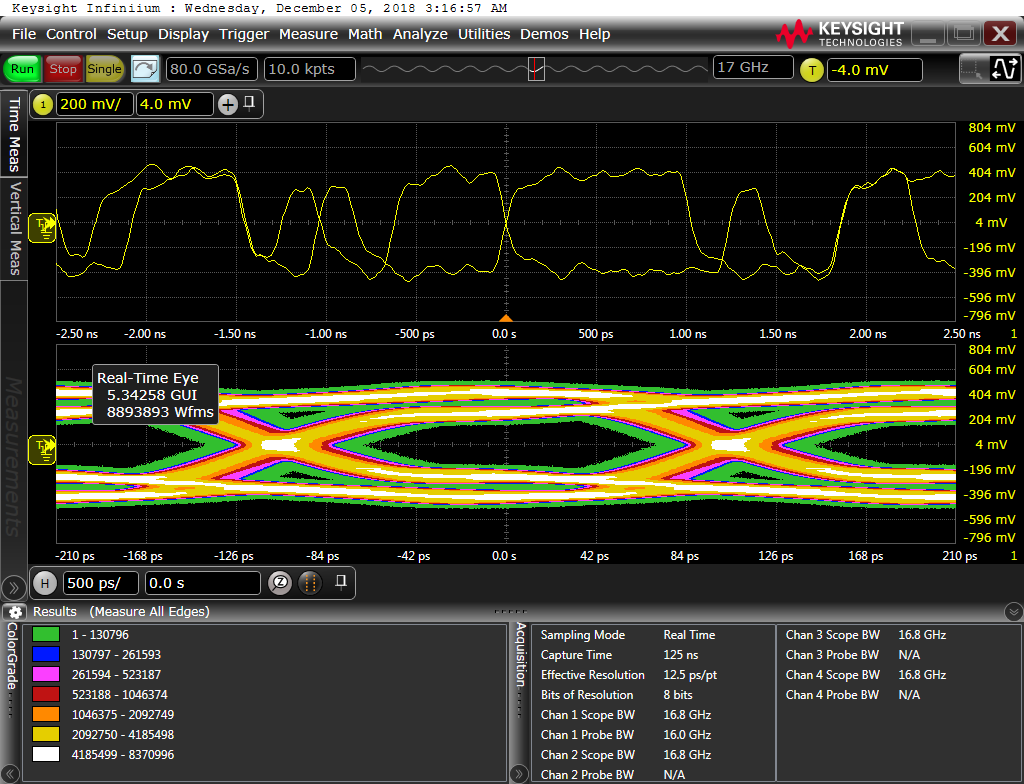
\includegraphics[width=0.85\textwidth]{./figs-ut-upgrade/dcb/dcb_eye_diagram.png}
    \caption{
        An eye diagram for DCB, produced overnight.
        Wide-open and has no noise in the eye, an indication of good signal
        quality.
    }
    \label{fig:dcb-eye}
\end{figure}

Due to the nature of PRBS, once a single bit is received from the sequence,
the next bits can be predicted and checked against indefinitely.
A high-statistic check of PRBS is performed for 5 consecutive days without
a single bit error, corresponding to an error-free data transmission of
$\mathcal{O}(10^{15})$ bits in a low radiation environment\footnote{
    It was performed in our lab in the 3rd floor of PSC.
}.


\subsection{Quality assurance of DCB at CERN}
\label{dcb-qa}

There are $\sim 250$ DCBs shipped to CERN;
all of them has been tested at Maryland.
The author was tasked to perform a quality assurance procedure again on all of
them to ensure there is no damage due to shipping.
The author stitched a testing panel,
displayed in \cref{fig:dcb-cern-test-panel},
to perform the following tests,
similar to tests performed at Maryland,
with a single click\footnote{
    This made the author's life slightly easier.
    It also allowed the author to partially offload the task to volunteers.
    Thank you Roberto Piandani and Marian Stahl!
} on 2 DCBs at a time:

\begin{enumerate}
    \item Read the status of master GBTx to ensure the bi-directional
        connections are established.

    \item Perform a PRBS test with a DCB-generated PRBS for 2 minutes.
    \item If there is any error, the VTTx transmission bias current is
        increased from 5~mA to 6~mA, and the PRBS test is repeated.
    \item The thermistors connected to the GBT-SCA ADC are readout and checked
        to make sure they fall within a reasonable range.
\end{enumerate}

\begin{figure}[!htb]
    \centering
    \begin{subfigure}[t]{0.4\textwidth}
        \centering
        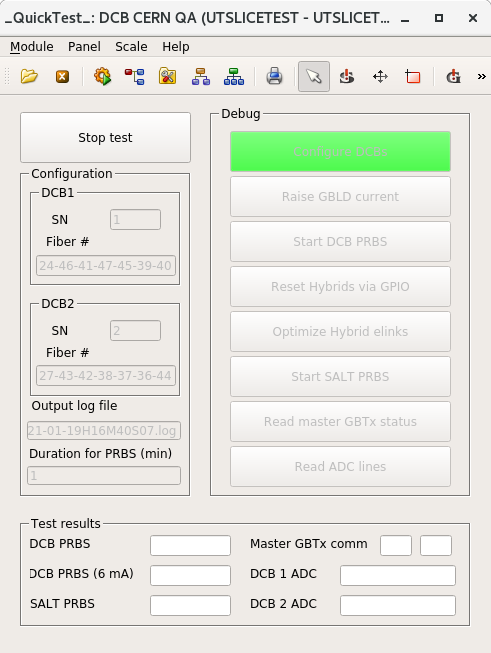
\includegraphics[width=\textwidth]{./figs-ut-upgrade/dcb/dcb_cern_panel_1.png}
        \caption{
            A running panel.
        }
    \end{subfigure}
    \hspace{24pt}
    \begin{subfigure}[t]{0.4\textwidth}
        \centering
        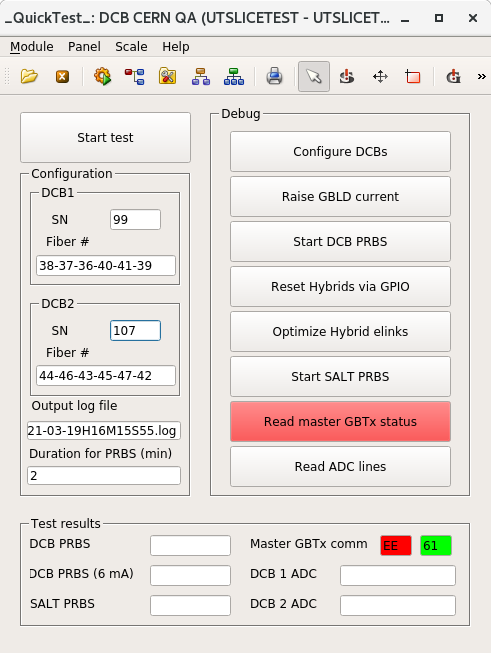
\includegraphics[width=\textwidth]{./figs-ut-upgrade/dcb/dcb_cern_panel_2.png}
        \caption{
            ...sometimes the master GBTx refuses to talk.
        }
    \end{subfigure}

    \caption{
        DCB CERN testing panel.
    }
    \label{fig:dcb-cern-test-panel}
\end{figure}

The panel is written in a pseudo C\# language used by the WinCC OA
SCADA (supervisory control and data acquisition) system,
the control system chosen by CERN.
The underlying functionalities are borrowed from code written by Mark Tobin
and other CERN experts.


\section{The LHCb online system}
\label{ref:ut:online}

The LHCb online system is responsible for ensuring a consistent clock
distribution across the whole detector, collecting readout data from front-end
electronics (FE) and filtering events with software-based HLT algorithms,
and provisioning initialization, control, and monitoring of the detector.
%%%%
As shown in \cref{fig:lhcb-online},
aside from execution of HLT algorithms,
the LHCb online system consists of three important components:
\cite{Colombo_2018}:

\begin{figure}[!htb]
    \centering
    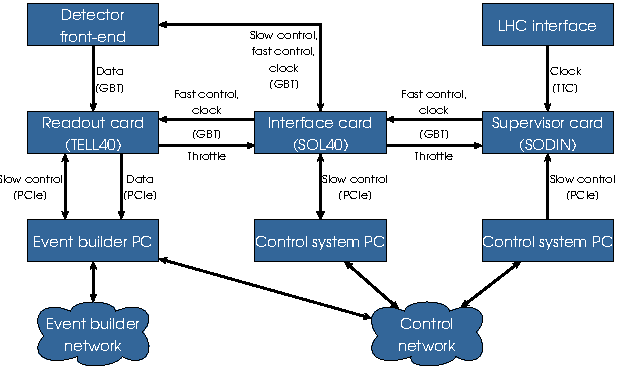
\includegraphics[width=0.8\textwidth]{./figs-ut-upgrade/online/lhcb_online_sys_overview.pdf}
    \caption{
        An overview of the LHCb online system.
    }
    \label{fig:lhcb-online}
\end{figure}

\begin{itemize}
    \item \textbf{SODIN}:
        A central readout manager that receives clock from the LHC and
        distributes it to SOL40.
        It also issues Timing and Fast Control (TFC) commands\footnote{
            In general, TFC commands have the following capability:
            Provide a bunch-crossing ID at 40~MHz to FE which is used to ensure
            synchronicity across FE in the detector;
            allow FE to operate in special modes such as producing a calibration
            pulse or transmitting data non-zero-suppressed;
            instruct FE to reset their operation logic while retaining their
            configuration;
            among others.
            More information regarding TFC can be found at
            \cite{Alessio:1424363} but is not the focus of this text.
        } to the front-end to regulate data flow.

    \item \textbf{SOL40}:
        Fan out TFC commands to TELL40 and FE,
        and fan in throttle from TELL40 to SODIN.
        It also provides an interface between the FE and the control system of
        the experiment.

    \item \textbf{TELL40}:
        Readout from FE. Hosted inside event builders.
        Accept TFC commands for synchronization.
\end{itemize}

The functionalities required by the three components is implemented with a
single hardware:
the PCIe40 board,
which is a PCI Express Gen 3.0 x16 add-in card based on Intel Arria 10 FPGA and
high-density optical I/O with up to 48 duplex GBT link ports.
By flashing a different firmware,
a PCIe40 can satisfy the requirements by each component.
In its TELL40 flavor, PCIe40 is capable of copying the received readout data
into the main system memory at over 100~Gb/s.
It is also possible to load a firmware combining all three components with
reduced read bandwidth, in which case the PCIe40 forms the foundation of the
MiniDAQ system used by the collaborating institutions to develop FE
\cite{GranadoCardoso:2702137}.

The remaining section first provides an overview of
the slow control protocol (\cref{online-dim}),
followed by an introduction on the MiniDAQ system
(\cref{online-minidaq}).
Finally, a program developed in-house is discussed in \cref{online-nanodaq},
showing its utilities in testing FE at Maryland.


\subsection{The \dim control protocol}
\label{online-dim}

The Distributed Information Management (\dim) system provides
a network\footnote{
    With TCP/IP protocol.
} based inter-process communication protocol \cite{Gaspar:559279},
implemented in C to ensure portability across operating systems,
which the slow control system is based upon.
The \dim protocol requires a central name server (like a phone directory)
which all \dim server (like people) implementing controlling of devices will
register on.
When the controller, a \dim \emph{client}, need to configure a device with a
certain name,
it first inquire the name server (look up a name in the phone
directory) before connecting to the specific \dim server and effecting changes
(call the people listed in the directory and do things).

To be more specific,
first consider a single SOL40 connected to some FE:
A part of the FPGA on the PCIe40 card implements a GBT transceiver.
Further, the ability to write to and read from that transceiver is exposed
to the operating system\footnote{
    Typically linux, more specifically CentOS 7.
} on SOL40.
A \dim server is also running on the SOL40 to translate different types of GBT
write/read commands,
such as GBT-I2C and GBT-GPIO,
to \dim \emph{services}.

\begin{figure}[!htb]
    \centering
    \hspace{0.2em}
    \resizebox{0.75\columnwidth}{!}{
        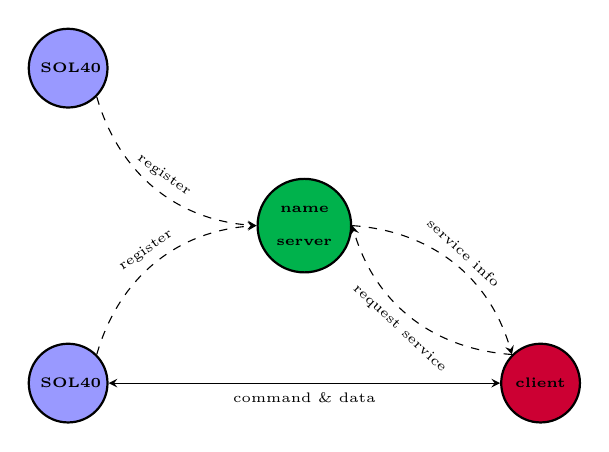
\begin{tikzpicture}[
        dim/.style = {
            draw, thick,
            circle,
            text = black,
            font = \bfseries,
            minimum size = 0.7,
            text width = 2em,
            align = center,
        }
    ]
    \node[dim,fill=blue!40!white] (1) at (-3, -2) {\tiny SOL40};
    \node[dim,fill=blue!40!white] (2) at (-3,  2) {\tiny SOL40};

    \node[dim,fill=blue!30!green] (3) at ( 0,  0) {\tiny name server};
    \node[dim,fill=blue!20!red]   (4) at ( 3, -2) {\tiny client};

    \path[-stealth,dashed] (2.south east)
        edge[bend right=35] node[midway,above,rotate=-35] {\tiny register}
        (3.west);
    \path[-stealth,dashed] (1.north east)
        edge[bend right=-35] node[midway,above,rotate=35] {\tiny register}
        (3.west);

    \path[-stealth,dashed] (4.north west)
        edge[bend left=35] node[midway,below,rotate=-43] {\tiny request service}
        (3.east);
    \path[-stealth,dashed] (3.east)
        edge[bend left=35] node[midway,above,rotate=-43] {\tiny service info}
        (4.north west);

    \path[>=stealth,<->] (4.west)
        edge node[midway,below] {\tiny command \& data}
        (1.east);
\end{tikzpicture}

    }
    \hspace{0.2em}
    \caption{
        A diagram illustrating \dim control flow.
    }
    \label{fig:dim-lhcb}
\end{figure}

Each SOL40 then registers its \dim services to a central name server.
A human controller sitting in the control room at point 8 will have a computer
running a \dim client with many clickable buttons corresponding to GBT write
commands to different FE.
The controller can click a button in which case the \dim client will perform
a lookup on the central name server and make changes to the FE via the
\dim server running in the looked-up SOL40.
The procedure is illustrated in \cref{fig:dim-lhcb}.
Each \dim service declares its communication interface as a string to the \dim
sever, with the interface described as the following:

\begin{lstlisting}
    <input type>:<number of inputs>;<return type>:<number of returns>
\end{lstlisting}
where:

\begin{itemize}
    \item The following types are allowed:
        Char (\lstinline{C}): 1 byte;
        Int (\lstinline{I}): 4 bytes;
        Long (\lstinline{L}): 4 bytes;
        Short (\lstinline{S}): 2 bytes;
        Double (\lstinline{D}): 8 bytes;
        Float (\lstinline{F}): 4 bytes;
        Long Long (\lstinline{X}): 8 bytes.
    \item The return value is optional so that interface of the form
        \lstinline{I:2} is legal.
    \item The return value (only) can have variable lengths in which case
        the \lstinline{number of returns} is omitted.
\end{itemize}

In LHCb it is often the case that ASIC register addresses and the values to
write are transmitted with a number of Chars.


\subsection{MiniDAQ}
\label{online-minidaq}

The MiniDAQ system,
a miniature LHCb online system,
is provided by the LHCb collaboration as a development
platform for all front-end electronics \cite{GranadoCardoso:2702137}.
The MiniDAQ hardware is an off-the-shelf server equipped with a PCIe40 card.
The PCIe40 card, shown in \cref{fig:pcie40}, is loaded with a firmware capable
of performing triple duty of SODIN, SOL40, and TELL40.
To form a complete package, MiniDAQ provides the following software:

\begin{figure}[!htb]
    \centering
    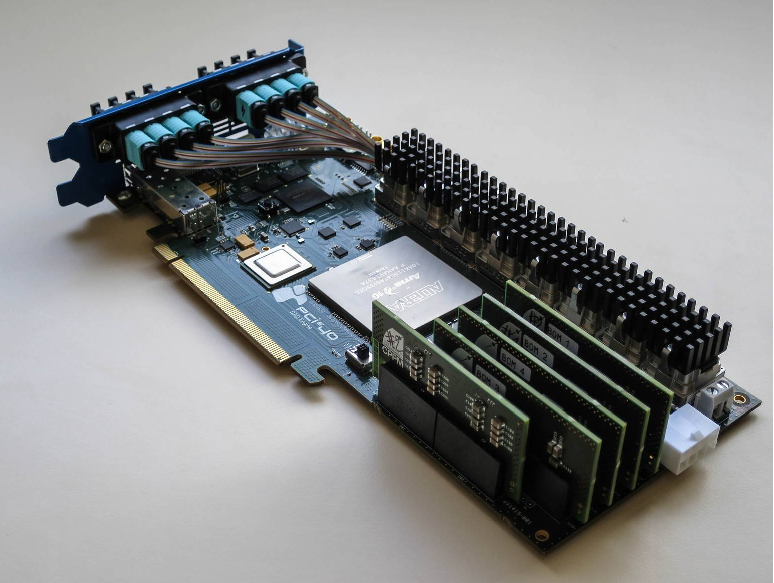
\includegraphics[width=0.75\textwidth]{./figs-ut-upgrade/online/pcie40.pdf}
    \caption{
        A prototype PCIe40 card.
    }
    \label{fig:pcie40}
\end{figure}

\begin{itemize}
    \item A linux distribution, typically CentOS 7.
    \item A linux kernel module to interface the PCIe40 FPGA to the operating
        system.
    \item A \dim server named \smalltt{gbtserv}. A \dim name server is also
        provided.
    \item A WinCC OA project acting as a control system more geared toward
        development.
        The \dim client is incorporated into WinCC OA by the JCOP framework,
        developed in-house at CERN.
\end{itemize}

The WinCC OA project on the MiniDAQ provides functionalities such as programming
the data GBTxes with GBT-I2C protocol,
shown in \cref{fig:wincc-oa-gbt},
and monitoring the readout from them,
shown in \cref{fig:wincc-oa-memmon}.
These functionalities are crucial in the early states of the DCB development and
validation,
but becomes increasingly cumbersome as the focus shifts on quality assurance
of a large number of production DCBs.

\begin{figure}[!htb]
    \centering
    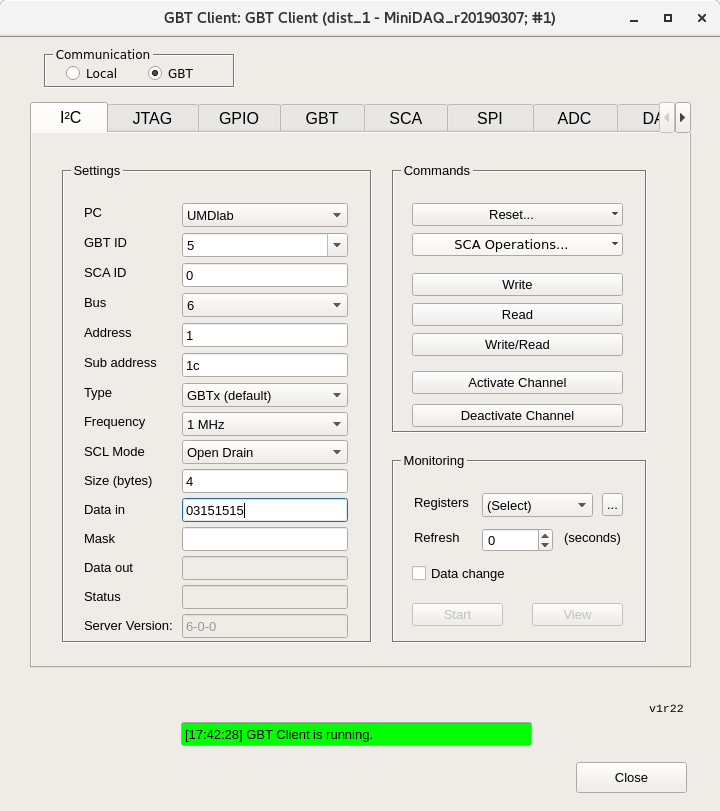
\includegraphics[width=0.7\textwidth]{./figs-ut-upgrade/online/gbt_client_slave_gbt_i2c_test.png}
    \caption{
        The WinCC OA MiniDAQ projection interface to program a single data GBTx.
        It supports both programming individual registers (as shown in this
        figure) or programming all registers with a text file.
    }
    \label{fig:wincc-oa-gbt}
\end{figure}

\begin{figure}[!htb]
    \centering
    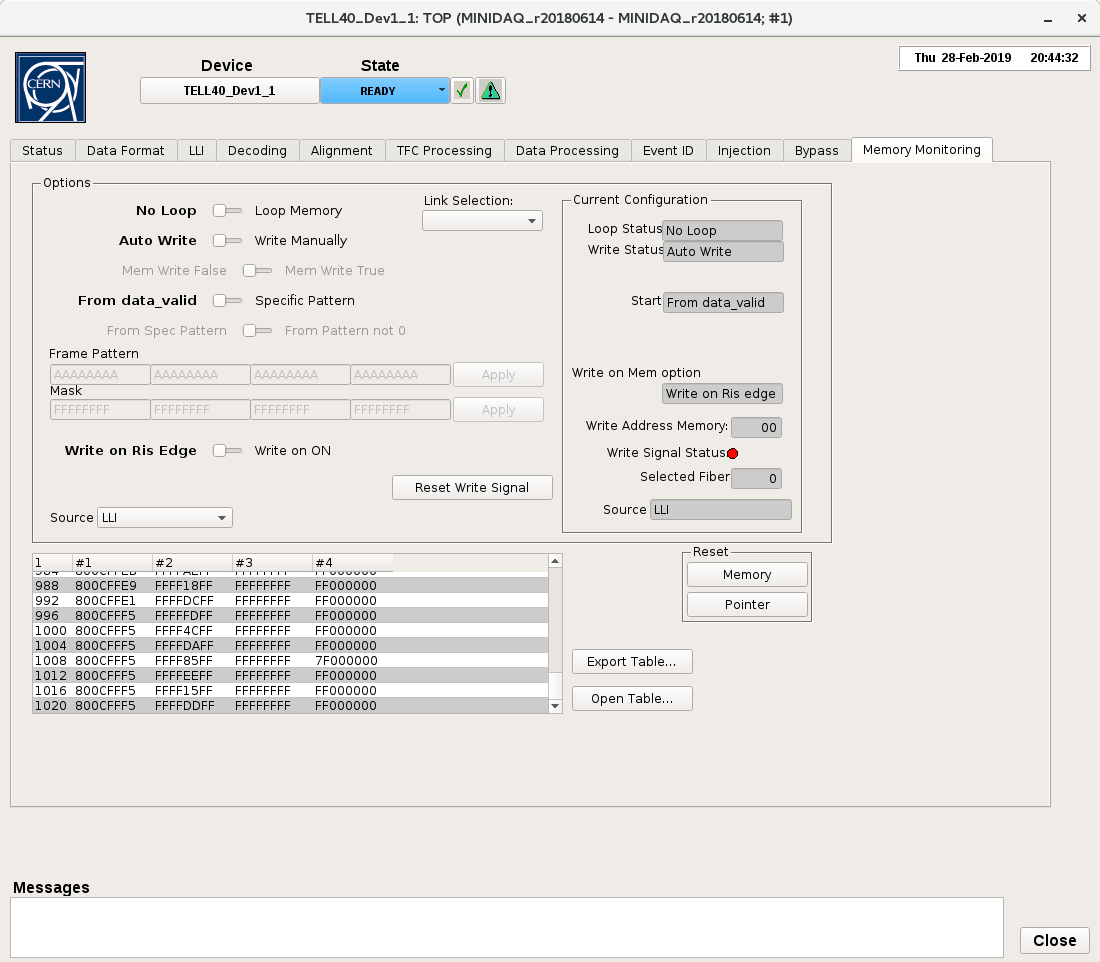
\includegraphics[width=0.7\textwidth]{./figs-ut-upgrade/online/memory_monitoring_panel.png}
    \caption{
        A WinCC memory monitoring panel.
    }
    \label{fig:wincc-oa-memmon}
\end{figure}


\subsection{\nanoDAQ: A reverse-engineered \dim client for testing UT electronics}
\label{online-nanodaq}

As stated in the previous section, repeated testing with the official MiniDAQ
project is hard.
Here the author supplies two concrete examples:

\begin{itemize}
    \item A DCB contains 6 data GBTxes.
        With the official control panel, shown in \cref{fig:wincc-oa-gbt},
        programming 6 data GBTxes to do PRBS tests requires the author change
        the ``Address'' field from 1 to 6 manually 6 times.

    \item As a stave with SALTs arrived at Maryland,
        a full readout test for every DCB becomes possible.
        As discussed in \cref{dcb-gbt-link},
        each e-link phase needs to be adjusted to ensure stable readout,
        which is performed on every turn on.

        The procedure is the following: First configure the SALT to output a
        fixed pattern\footnote{
            For some reason, the pattern \smalltt{C4} was chosen.
        }, then stare at the memory monitoring panel,
        displayed in \cref{fig:wincc-oa-memmon},
        to spot the unstable e-links, and adjust phases for each e-link until
        they are stable.

        The procedure was further complicated by a bug in the panel
        shown in \cref{fig:wincc-oa-memmon}:
        To start reading the memory which are filled with GBT frames from the
        GBTxes, the option ``Write on Ris Edge'' needs to be toggled to on. To
        inspect these readouts, it needs to be toggled off. There is a chance
        that the switch auto-toggles in which case the only known workaround to
        the author is clicking on the switch repeatedly until it stops.
\end{itemize}

It is evident that a batch-processing program to perform these procedures with
few clicks or a single command is highly desirable.
Unfortunately programming with WinCC OA is hard:
the development environment, called \lstinline{gedi}, can auto-complete
some of the keywords but cannot check basic errors such as an undefined
variable.
This resulted in frequent typos in the source code that are hard to spot and
debug.

In the end,
noting that the MiniDAQ comes with a \dim server that is responsible for
performing all GBT-related tasks,
the author decided to write a command line \dim client with Python.
First, all registered \dim services are dumped with \pydim
\cite{pydim}.
Then, the required functionalities such as I2C, GPIO, and memory
monitoring are searched for based on names.
For example, some of the I2C services have the following signatures:

\begin{lstlisting}
    Service 22436 : Type of service = 1 name = Gbt/UMDlab/SrvcI2CWrite, format = I:1
    Service 26017 : Type of service = 1 name = Gbt/UMDlab/SrvcI2CRead, format = I:1;C
    Service 24492 : Type of service = 2 name = Gbt/UMDlab/CmndI2COperation, format = C:128;C
\end{lstlisting}

It became possible to identify these services in the JCOP and \smalltt{gbtserv}
source code,
and understand the required arguments.
Hence the \nanoDAQ project \cite{nanoDAQ} is born.
The name suggests that it only implements a small fraction of the capabilities
provided by MiniDAQ, namely I2C, GPIO, and memory monitoring readout.

With \nanoDAQ, multiple DCBs (in the example below 3) can be configured
\emph{programmatically} to generate PRBS patterns,
for example by running the following \smalltt{bash} script:

\begin{lstlisting}[language=Bash]
    #!/usr/bin/env bash
    GBTLINKS=( 3 4 5 )

    for i in ${GBTLINKS[@]}; do
        echo "Reset all data GBTxs first..."
        ./dcbutil.py gpio --reset $i

        echo "Initialize DCB on GBT link $i..."
        # here a configuration file is loaded
        ./dcbutil.py init ./gbtx_config/slave-Tx-wrong_termination.txt -g $i

        echo "Configure each data GBTx to do PRBS..."
        ./dcbutil.py write 1c 3 -g $i -s 1 2 3 4 5 6
        # to flip back to normal operation:
        #./dcbutil.py write 1c 1 -g $i -s 1 2 3 4 5 6
    done
\end{lstlisting}

\nanoDAQ also comes with an e-link phase adjusting script, which performs the
following tasks in sequence,
with a demo screenshot provided in \cref{fig:nanodaq-phaseadj}:

\begin{enumerate}
    \item Configure all SALTs connected.

    \item Perform an initial scan of the e-link readout,
        and ask the user to input the e-link indices to adjust.

    \item Loop over all possible DCB e-link phases, and save the readout for
        each of them.
        The stability of the readout for a given phase is determined by checking
        if all readout Bytes can be shift to the fixed pattern
        \smalltt{C4} with a common phase\footnote{
            Consider the pattern \smalltt{0x13}, which can be written in binary
            form as \smalltt{0b00010011}.
            Compare this to the binary form of \smalltt{0xC4} which is
            \smalltt{0b11000100},
            noting that the input stream is a series of Bytes of the form
            \smalltt{0b000100[11,000100]11...},
            it can be concluded that \smalltt{0x13} can reproduce \smalltt{0xC4}
            by shifting the pattern start 6 Bytes to the right.
        }.
        If not, but if the most common pattern in the readout data is a phase
        shift,
        the phase is marked in \textcolor{orange}{\bfseries yellow};
        otherwise it is marked with a \textcolor{red}{\bfseries red ``X''}.

    \item A stable phase,
        marked in \textcolor{olive}{\bfseries green},
        is determined for each e-link by picking
        the central phase of consecutive stable phases.

    \item Adjust both the DCB e-link phases and the SALT output phase
        to ensure the output pattern is \smalltt{C4}.
\end{enumerate}

\begin{figure}[!htb]
    \centering
    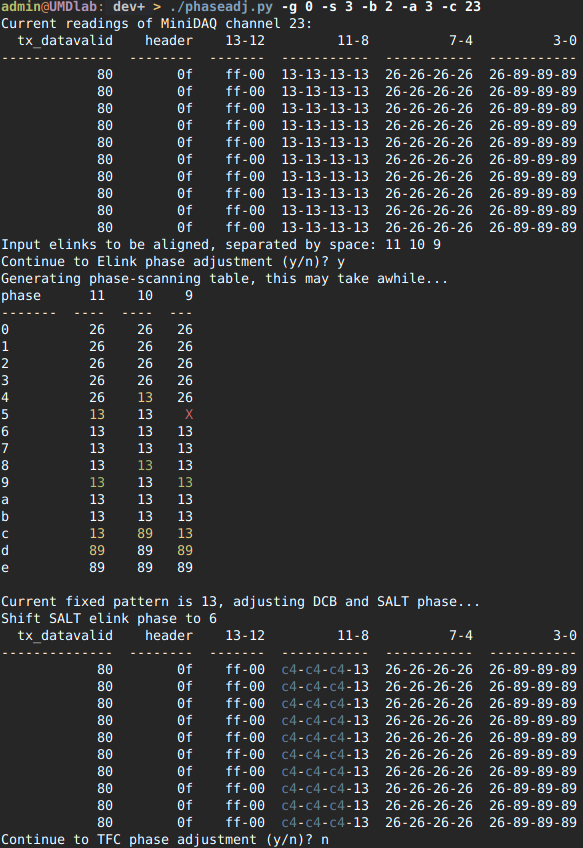
\includegraphics[width=0.75\textwidth]{./figs-ut-upgrade/online/elk_phase_adj.png}
    \caption{
        E-link phase adjust with \nanoDAQ.
    }
    \label{fig:nanodaq-phaseadj}
\end{figure}

Looking back, the author gained most of the online system knowledge due to the
pain inflicted by DCB and SALT testing.
